%
% main.tex
%

% notes = hide | show | only
\documentclass[xcolor=dvipsnames,dvip,notes=show,table]{beamer}

% Para crear una versión 'handout' (impresa)
%\documentclass[xcolor=pst,dvips,handout,notes=show]{beamer}

%
% cabeceras.tex
%
% Copyright 2003, Diego Berrueta Muñoz
%
% Cabeceras comunes
%

\usepackage[T1]{fontenc}

%Glosario

\usepackage[toc,style=treenoname,order=word,counter=section]{glossaries}

\usepackage{xspace}


\usepackage{tikz,times}
\usetikzlibrary{mindmap,backgrounds}

% cambia algunas fuentes (utilidad dudosa)
\usepackage[scaled=0.92]{helvet}
\usepackage{pifont}
\usepackage{courier}

% cambia algunas fuentes en modo matemático a Palatino
\usepackage{mathpazo}

% españolización
\usepackage[spanish]{babel}
\usepackage[utf8]{inputenc}
%\extrasspanish

% gráficos y colores
\usepackage{rotating}
\usepackage{graphicx}
\usepackage{color}
%\usepackage[all]{xy}
%\usepackage{pstricks}
\usepackage{pst-node}
%\usepackage[dvips,usenames]{pstcol}
%\usepackage{pdftricks}
%\usepackage{pst-uml}  % para hacer diagramas UML
%\usepackage{rail}     % para hacer diagramas de gramáticas

% mejoras visuales
\usepackage{enumerate}
\usepackage{fancyhdr}  % para configurar los encabezados
\usepackage{fancybox}  % para hacer cajitas
\usepackage[normal,oneline,sf,bf]{caption2}
\usepackage{titlesec}  % para configurar los títulos de sección
\usepackage{paralist}


\usepackage{epigraph}

% citas, referencias e índices
\usepackage{cite}
%\usepackage{citesort}   % da errores al compilar
\usepackage{makeidx}

% incrustaciones de código fuente
%\usepackage[norules,nolineno]{lgrind}
\usepackage{verbatim}
\usepackage{listings}
%\usepackage{noweb,a4wide}


%\usepackage{textcomp}
\usepackage[right]{eurosym}

% columnas
\usepackage{multicol}

% tablas
\usepackage{longtable}
%\usepackage{ltxtable}

% impresión elegante de URLs
\usepackage{url}

\makeatletter
\def\url@pfcstyle{%
  \@ifundefined{selectfont}{\def\UrlFont{\sf}}{\def\UrlFont{\small\ttfamily}}}
\makeatother
%% Now actually use the newly defined style.
\urlstyle{pfc}


% márgenes
\usepackage[a4paper, left=30mm, right=20mm, top=25mm, bottom=25mm]{geometry}
%\usepackage[a4paper, left=20mm, right=20mm, top=25mm, bottom=25mm]{geometry}

% 
% \usepackage[a4,center,cam]{crop}
\usepackage{blindtext}

% salida en PDF navegable
%\usepackage{hyperref}
\usepackage[plainpages=false,colorlinks, linkcolor=black]{hyperref}

% quitar en versión final
%\usepackage{showkeys}   % depuración de etiquetas y referencias
%\usepackage{showidx}    % depuración de índice

% configuración del paquete "listings"

\lstset{%
        %language=Java,
	basicstyle=\footnotesize\sffamily,
	keywordstyle=\bfseries, %\color{darkred}
 	stringstyle=\itshape, %\color{violet}
 	commentstyle=\itshape, %\color{blue}
 	showspaces=false,
 	showtabs=false,
 	showstringspaces=false,
 	frame=trBL,
        frameround=tttt,
        %backgroundcolor=\color{lightyellow},
	inputencoding=utf8,
 	extendedchars=true,
 	numbers=none,
        aboveskip=0.5cm,
        belowskip=0.5cm,
        xleftmargin=1cm,
        xrightmargin=1cm,
	breaklines=true
}
\definecolor{darkred}{rgb}{0.5, 0, 0}
\definecolor{violet}{rgb}{1, 0, 1}
\definecolor{lightyellow}{rgb}{1,1,0.8}


%%%%%%%%%%%%%%%%%%%%%%%%%%%%%%%%%%%%%%%%%%%%%%%%%%%%%%%%%%%%%%%%%%%%%%
% cabeceras y pies de página (con el paquete "fancyhdr")
\headheight 15pt
%\addtolength{\headwidth}{\marginparsep}
%\addtolength{\headwidth}{\marginparwidth}
%\renewcommand{\chaptermark}[1]{\markboth{\MakeUppercase{#1}}{}}
%\renewcommand{\sectionmark}[1]{\markright{\thesection\ #1}}
%\fancyhead[LE,RO]{\textbf{\thepage}}
%\fancyhead[RE]{\textit{\leftmark}}
%\fancyhead[LO]{\rightmark}
%\fancyfoot[LCR]{}
\fancyhead{} % Todos los campos en blanco en la cabecera
\fancyfoot{} % Lo mismo al pie
\fancyhead[RO, LE]{\thepage}
\fancyhead[LO, RE]{\slshape\leftmark}
\renewcommand{\headrulewidth}{0.5pt}
\renewcommand{\footrulewidth}{0.5pt}


%%%%%%%%%%%%%%%%%%%%%%%%%%%%%%%%%%%%%%%%%%%%%%%%%%%%%%%%%%%%%%%%%%%%%%
% títulos de secciones (con el paquete "titlesec")
\titleformat{\chapter}[display]
	{\fontfamily{pag}\selectfont\Huge}
	{\LARGE\chaptertitlename\ \thechapter}{20pt}{\bfseries}
\titleformat{\section}
	{\fontfamily{phv}\selectfont\LARGE}
	{\thesection}{1em}{\bfseries}[\titlerule]
\titleformat{\subsection}
	{\fontfamily{phv}\selectfont\Large}
	{\thesubsection}{1em}{\bfseries}
\titleformat{\subsubsection}
	{\fontfamily{phv}\selectfont\large}
	{\thesubsubsection}{1em}{\bfseries}


%%%%%%%%%%%%%%%%%%%%%%%%%%%%%%%%%%%%%%%%%%%%%%%%%%%%%%%%%%%%%%%%%%%%%%
% espaciado entre párrafos
\addtolength{\parskip}{+0.2cm}


%%%%%%%%%%%%%%%%%%%%%%%%%%%%%%%%%%%%%%%%%%%%%%%%%%%%%%%%%%%%%%%%%%%%%%
% salida en PDF navegable (con el paquete "hyperref")
\hypersetup{bookmarks,
	bookmarksnumbered,
%	colorlinks, % quitar en las versiones impresas
	hyperindex,
	%linkcolor=red,
	%anchorcolor=black,
	%citecolor=green,
	citecolor=violet,
	%filecolor=magenta,
	%menucolor=red,
	%pagecolor=red,
	%urlcolor=cyan,
	pdftitle={PhD. Dissertation-Jose María Alvarez Rodríguez},
	pdfauthor={Jose María Alvarez Rodríguez}
	pdffitwindow,
	plainpages=false,
	pageanchor=false,
	pdfstartview={}}


%%%%%%%%%%%%%%%%%%%%%%%%%%%%%%%%%%%%%%%%%%%%%%%%%%%%%%%%%%%%%%%%%%%%%%
% profundidad de secciones y numeración
%\setcounter{tocdepth}{4}
\setcounter{secnumdepth}{3}


%%%%%%%%%%%%%%%%%%%%%%%%%%%%%%%%%%%%%%%%%%%%%%%%%%%%%%%%%%%%%%%%%%%%%%
% división silábica
\hyphenation{pu-bli-ca-ción con-tex-tua-li-za-ción pro-ble-mas Mi-nis-te-rio li-ci-ta-ción si-guien-tes desa-rro-llar con-tra-ta-ción pan-europea fa-ci-li-tar in-ter-opera-bility
 elec-tró-ni-ca li-ci-ta-do-ras he-te-ro-gé-neos res-trin-gi-do cons-cien-te de-sa-rro-lla-da mo-de-lo paí-ses ge-ne-ra-da
 par-ti-ci-pa-ción ad-mi-nis-tra-ti-vos bi-blio-gra-fía re-gis-tra-do-ra ad-mi-nis-tra-ti-va ca-rac-te-rís-ti-cas
 Pa-ra-le-la-men-te des-cri-ben vo-ca-bu-la-rio me-dian-te do-cu-men-to di-fe-ren-tes bi-blio-gra-fía mo-de-lo
 ve-ri-fi-ca rea-li-zar res-tric-ciones Por ejem-plo su-ge-ren-cias mo-de-los rea-li-za si-guien-do he-te-ro-gé-neas ello
 ra-zo-na-ble li-mi-ta-cio-nes reu-ti-li-cen ini-cia-ti-va va-ria-da exis-ten ob-te-ner con-ti-nua-men-te me-dian-te ins-ti-tu-ción
 pro-pues-ta pu-bli-ca-ción ca-tá-lo-go mo-ni-to-ri-za-ción vi-sua-li-za-ción mo-de-los co-rres-pon-dien-tes
 re-fe-ren-cia re-la-ti-vas par-ti-cu-lar  ele-men-to mo-de-la-do se-le-ccio-na-do pro-du-cción Re-con-ci-lia-ción des-crip-cio-nes broader-Transitive 
 de-pen-dien-do Ca-tá-lo-gos vo-ca-bu-la-rios Pro-pie-ta-rio des-plie-gue De-sa-rro-lla-dor mo-de-lar res-pues-ta si-mi-la-res rea-li-za-do SE-RI-MI 
Evol-ving ha-bi-li-tar rea-li-za-ción pu-bli-ca-ción ge-ne-ra-ción rea-li-za-ban ac-tua-li-za-ción ac-ce-so ha-cer es-tán-dar 
vo-ca-bu-la-ry con-si-de-ra-do des-cri-bir pu-bli-car pu-bli-ca-dos ta-xo-nó-mi-ca Pro-duct-on-to-lo-gy Va-lo-res in-terope-ra-bi-li-dad MOL-DEAS 
man-te-ni-mien-to re-pre-sen-tar ta-xo-no-mías des-crip-ción ge-ne-ra cons-truc-ción re-pre-sen-tan-do rea-li-za-das trans-fe-ren-cia 
uti-li-za-ble pu-bli-ca be-ne-fi-cios res-pon-sa-bi-li-da-des rea-li-zan Ad-mi-nis-tra-ción con-ti-nua-ción prio-ri-ta-rio ICT 
in-terope-ra-ble ge-ne-ra-do con-fi-gu-ra-cio-nes rea-li-zan-do rea-lis-ta má-xi-mo Cons-ti-tu-yen-do pro-ble-ma po-si-bi-li-dad ma-yor coo-pe-ra-ción 
ra-zo-na-mien-to Des-crip-tion con-cep-tua-li-za-ción de-sa-rro-lla-dos ope-ra-do-res axio-mas go-bier-no or-ga-nis-mos éxi-to 
si-guien-te do-mi-nios pro-duc-ción Na-tio-nal orien-ta-da ló-gi-ca in-di-vi-duos di-se-ña-do for-ma-li-za-dos ta-xo-no-mía 
auto-má-ti-ca ca-li-dad re-co-men-da-ble ad-mi-nis-tra-ti-vo su-mi-nis-tre error ca-rac-te-rís-ti-ca ele-men-tos he-rra-mien-tas 
eva-lua-ción res-pec-to Ad-mi-nis-tra-cio-nes ex-pe-ri-men-tal orien-ta-das re-gis-tros do-cu-men-tos má-xi-ma je-rar-quía 
sa-tis-fac-to-rios obs-tan-te con-su-mi-dos con-fe-ren-cias SPARQL rea-li-za-dos va-lo-ran eco-no-mi-zar fle-xi-ble ex-pe-dien-te 
pro-ce-di-mien-to usan-do ame-ri-ca-nas fa-mi-lia ni-vel ra-zo-na-do-res re-pre-sen-ta-ción lo-ca-li-za-do Man-ches-ter 
en-ri-que-ci-mien-to he-rra-mien-ta rea-li-zar-se prio-ri-ta-rios Li-ci-ta-cio-nes ne-ce-sa-rios ma-te-ria-li-zan es-pe-cia-li-zán-do-se 
Com-pu-ting pla-ni-fi-ca-ción cua-li-ta-ti-va de-sa-for-tu-na-da-men-te li-de-ra-do ma-te-ria-li-za-do Cons-tructs 
ma-te-ria-li-za WESO en-ten-di-mien-to MOLDEAS ela-bo-ra-ción re-fe-ren-te re-gis-tra-tion uni-la-te-ral po-si-bi-li-tar ope-rar 
in-ter-ope-ra-bles ad-mi-nis-tra-ti-vas fle-xi-bi-li-dad auto-no-mía co-mer-cio procesa-miento de-sa-rro-llan-do meta-in-for-ma-ción 
apro-pia-dos li-mi-ta-do es-pe-cia-li-za-ción ló-gi-cas in-de-pen-dien-te-men-te ge-ne-ral dis-po-ner dis-mi-nu-yen-do co-rrien-te 
rea-pro-ve-char de-sa-rro-llo ge-ne-ral Ins-ti-tu-te com-pu-ting pos-te-rior con-su-mi-da mi-llo-nes Fi-gu-ras cons-tan-te equi-va-len-cia ope-ra-cio-nes 
fac-to-ri-za-ción Res-pon-sa-bles Geo-Linked-Data reu-ti-li-za-ción co-rrec-tos trans-for-ma-ción bien con-si-guien-te des-cu-brien-do 
geo-rre-fe-ren-cia-ción pro-li-fe-ra-ción cum-pli-mien-to Ne-go-tia-ted uti-li-dad ma-nual es-pe-cia-li-za-ción ma-yo-ría mo-de-la 
des-cu-bri-mien-to rea-li-za-da pu-bli-can se-lec-cio-nar me-ca-nis-mos fun-cio-na-li-dad ve-ri-fi-car ines-pe-ra-dos re-gis-tro 
pro-pues-tos trans-pa-ren-te va-ria-bles bi-blio-te-ca bi-blio-te-cas adap-ta-bi-li-dad in-ter-co-ne-xión va-ria-ble vi-sua-li-zar 
ope-ra-ti-vo ge-ne-rar su-mi-nis-tra-dos va-li-da-ción su-mi-nis-tra-dores pro-pie-da-des hi-po-ni-mia re-cu-pe-ra-dos in-de-pen-dien-te-ment-te 
triun-fo reu-ti-li-za-ción ge-ne-ral apro-xi-ma-ción va-ria-bi-li-dad teó-ri-cas con-ti-nuo di-se-ño des-afor-tu-na-da-men-te In-dus-trial prin-ci-pios 
di-fe-ren-cia-das eva-lua-dos re-qui-si-tos co-la-bo-ra-cio-nes co-la-bo-ra-ción in-dus-tria-les Se-venth pon-de-ra-do re-po-si-to-rios 
ex-pe-ri-men-ta-les pu-bli-ci-tar co-la-bo-ra-ción bi-llo-nes Doc-to-ra-do re-so-lu-ción cul-tu-ra-les trans-cur-so Pa-rro-quias Lo-gics co-rrec-to 
sig-ni-fi-ca-do Aña-dien-do ope-ra-ción ma-ne-ra agi-li-zar con-fian-za per-so-na-les in-al-te-ra-dos re-la-ti-vos des-cri-bien-do 
se-ña-la-das vo-ca-bu-la-ries con-tex-tua-li-za-da Ba-rras cir-cuns-cri-bién-do-se for-ma-li-za-ción fa-ci-li-tan-do re-ali-men-ta-ción 
re-fe-ren-cias ma-ni-fes-tar-se CKAN lo-ca-li-dad dia-gra-ma ver-da-de-ra-men-te es-ta-ble-ci-mien-to con-si-de-ra ta-reas co-rrec-ta 
co-he-ren-te pos-te-rior-men-te apro-pia-das exac-tos va-rios pro-pues-to ex-pe-ri-men-to re-fe-ren-tes orien-ta-dos ha-bi-tual con-cre-tas 
con-fi-gu-ran afi-lia-ción Gi-ner va-lo-ra-ción res-pon-sa-bi-li-dad}   

%%Tablas
\addto\captionsspanish{
        \def\listtablename{\'Indice de tablas}%
        \def\tablename{Tabla}} 

%%%Math
\usepackage{latexsym}
\usepackage{amsmath}
\usepackage{amssymb}
\usepackage{amsthm}

\usepackage{algorithm}
\usepackage{algorithmic}
\usepackage{multirow}
\usepackage{rotating}


\newtheorem{theorem}{Theorem}[section]
\newtheorem{proposition}[theorem]{Proposición}
\newtheorem{lemma}[theorem]{Lema}
\newtheorem{definition}[theorem]{Definición}
\newtheorem{examples}[theorem]{Ejemplos}
\newtheorem{remarks}[theorem]{Remarks}
\newtheorem{corollary}[theorem]{Corolario}
\newtheorem{remark}[theorem]{Remark}
\newtheorem{example}[theorem]{Ejemplo}
\newtheorem{conjecture}[theorem]{Conjecture}
\newtheorem{note}[theorem]{Nota}



\newsavebox\FrameBox
\newenvironment{Frame}{%
  \par\setbox\FrameBox\hbox\bgroup\minipage{0.9\textwidth}\parskip\baselineskip\ignorespaces
}{%
  \endminipage\egroup\fbox{\box\FrameBox}\par
}

\newcommand{\si}{$\oplus$\xspace}
\newcommand{\no}{$\ominus$\xspace}
\newcommand{\na}{$\odot$\xspace}


%Extraer
\newcommand{\linkeddata}{\textit{Linked Data}\xspace}
\newcommand{\opendata}{\textit{Open Data}\xspace}
\newcommand{\lod}{\textit{Linking Open Data}\xspace}
\newcommand{\ogd}{\textit{Open Government Data}\xspace}
\newcommand{\datasets}{\textit{datasets}\xspace}
\newcommand{\dataset}{\textit{dataset}\xspace}
\newcommand{\provenance}{\textit{provenance}\xspace}
\newcommand{\trust}{\textit{trust}\xspace}
\newcommand{\egov}{\textit{e-government}\xspace}
\newcommand{\pusi}{\textit{Public Sector Information}\xspace}
\newcommand{\gd}{\textit{Government Data}\xspace}
\newcommand{\wod}{Web de Datos\xspace}
\newcommand{\wode}{\textit{Web of Data}\xspace}
\newcommand{\eproc}{\textit{\gls{e-Procurement}}\xspace}
\newcommand{\gld}{\textit{Government Linked Data}\xspace}





%%%%%%%%%%%%%%%%%%%%%%%%%%%%%%%%%%%%%%%%%%%%%%%%%%%%%%%%%%%%%%%%%%%%%%

\title[MOLDEAS]{Métodos Semánticos de Reutilización de Datos Abiertos Enlazados en las Licitaciones Públicas}
\author[Jose María Álvarez Rodríguez]{\textbf{Tesis Doctoral presentada por} \\ \vspace{0.3cm} Jose María Álvarez Rodríguez \\ \vspace{0.35cm} Dirigida por\\ \vspace{0.15cm}Profesor Doctor D. José Emilio Labra Gayo}
\subtitle{}
\institute{Sistemas y Servicios Informáticos para Internet \\ Departamento de Informática \\ Universidad de Oviedo}


\date{Oviedo, 14 de Junio de 2012}

\begin{document}

\frame{
\titlepage

}

\frame{
\tableofcontents

}


%%%%%%%%%%%%%%%%%%%%%%%%%%%%%%%%%%%%%%%%%%%%%%%%%%%%%%%%%%%%%%%%%%%%%%
\section{Objeto de la Investigación}
\input{sections/objeto}
\section{Marco teórico y conceptual}
\input{sections/marco-teorico}
\section{Marco metodológico}
\frame{
\large
\begin{enumerate}
\setcounter{enumi}{2}
 \item Marco metodológico.
  \begin{itemize}
  \item Metodología de la Investigación.
  \item Definición del Ciclo de Vida para Datos Enlazados Abiertos.
  \item Aplicación del Ciclo de Vida al \textit{e-Procurement}.
  \item Creación del sistema MOLDEAS.
  \end{itemize}

\end{enumerate}

}


\frame{
  \frametitle{Metodología de la Investigación}

\begin{block}{Tipo}<1->
Investigación cuantitativa con base en evidencias empíricas.
Carácter descriptivo y comparativo.
\end{block}
\begin{exampleblock}{Diseño}<2->
\begin{enumerate}
 \item Definición Ciclo de Vida de Datos Enlazados Abiertos.
\item  Aplicación al dominio de \eproc.
\item  Creación del sistema MOLDEAS.
\item  Definición y ejecución de experimentos.
\end{enumerate}
\end{exampleblock}
}


\frame{
  \frametitle{Metodología de la Investigación}
\begin{alertblock}{Universo de Estudio}
Tres principales conjuntos de datos seleccionados:
\begin{enumerate}
\item Datos de anuncios de licitación (1 Millón) provistos por Euroalert.net desde 2008 a 2011.
\item Catálogos de Clasificaciones de Productos y Servicios (9: CPV, CPA, NAICS, etc.) provistos por UE, ONU, EEUU, etc.
\item Organizaciones, personas y países (clasificación NUTS de la UE).
\end{enumerate}
\end{alertblock}
}

\subsection*{Definición del Ciclo de Vida para Datos Enlazados Abiertos}

\frame{
  \frametitle{Visión General} 

\begin{figure}[htb]
\centering
  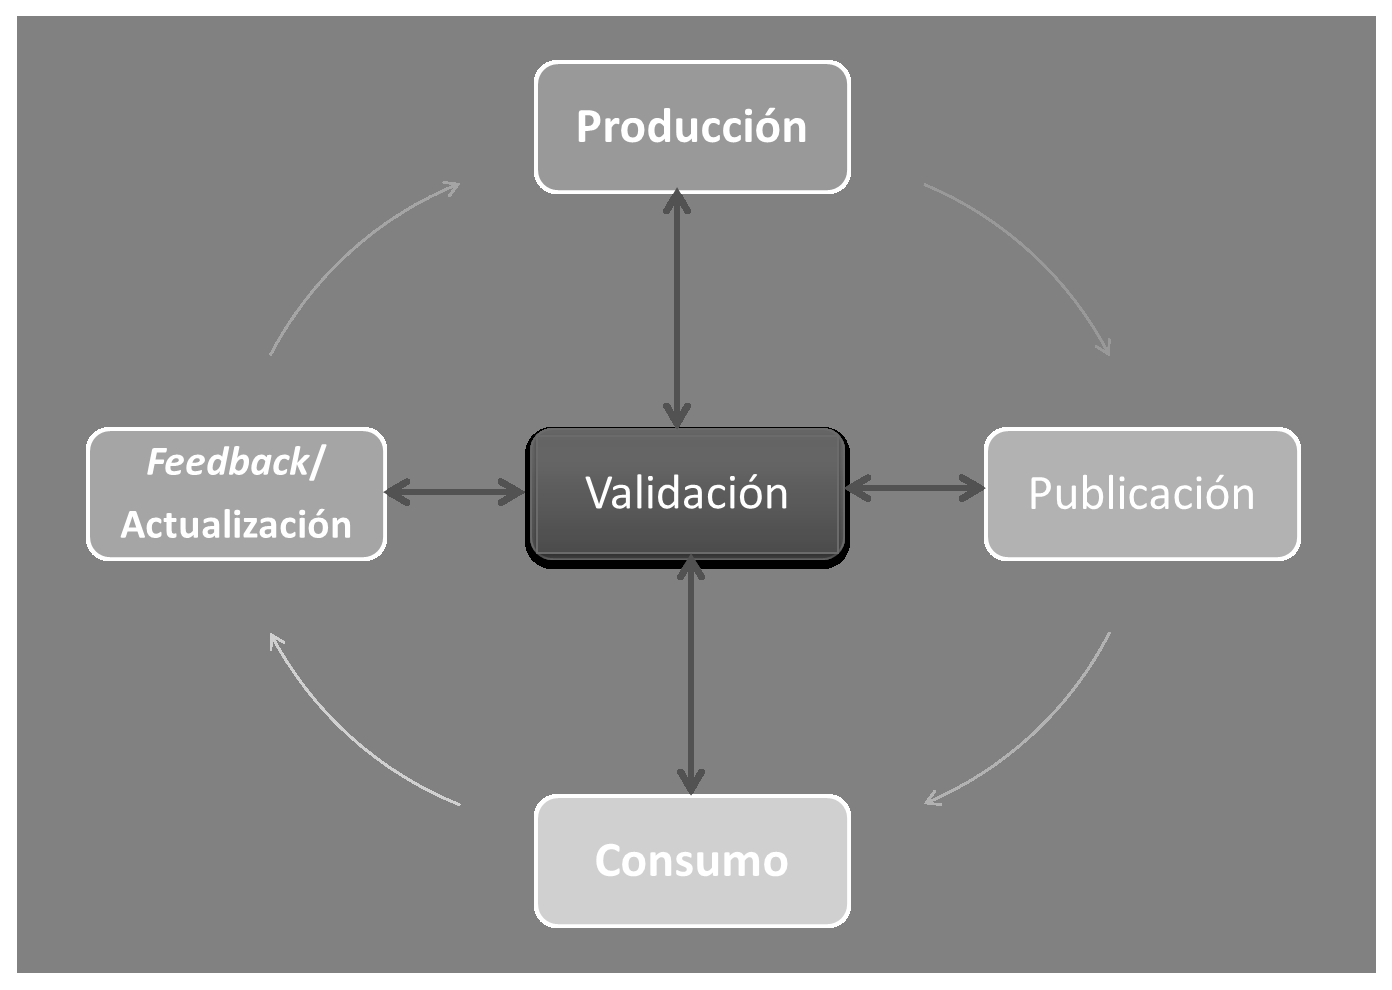
\includegraphics[width=8cm]{imgs/lld}
\caption{Procesos del Ciclo de Vida de Datos Enlazados Abiertos.}
\end{figure}

}


% 
% \frame{
%   \frametitle{Definiciones}
% 
% \begin{block}{Proceso $p$}<1->
% Se define un proceso $p$, como la aplicación de uno o varios métodos semánticos. 
% \end{block}
% 
% 
% \begin{exampleblock}{Método Semántico $sm$}<2->
% Se define un método semántico $sm$, como la consecución de $n$ tareas para llevar a cabo
% una operación sobre un \dataset. 
% 
% {\tiny El \dataset puede ser un conjunto de valores y datos $\mathcal{G}$, o bien
% un \dataset RDF, $\mathcal{D}$, dependiendo del proceso.}
% \end{exampleblock}
% 
% 
% \begin{alertblock}{Tarea $t$}<3->
%  Es cada uno de los pasos que se han de llevar a cabo para realizar un método semántico.
% \end{alertblock}
% 
% }



% \frame{
%   \frametitle{Proceso de Producción} 
% \begin{block}{Método Semántico de Producción}
% $SPM$ es una función que para un conjunto de tuplas de entrada o \dataset $\mathcal{G}$ y un conjunto de \textit{mapeos} $\mathcal{M}$  
% genera un \dataset RDF $\mathcal{D}$.
% \end{block}
% \begin{center}
%     $SPM : \mathcal{G} \times \mathcal{M} \longrightarrow \mathcal{D}$
% \end{center}
% 
% \begin{itemize}
%  \item Para todo valor $g_{i}$ del conjunto de entrada $\mathcal{G}$, existe al menos un
% \textit{mapeo} $m_{i}$ en el conjunto $\mathcal{M}$.
% \end{itemize}
% 
% }

% \frame{
%   \frametitle{Proceso de Publicación} 
% 
% \begin{block}{Método Semántico de Publicación}
% $S\mathcal{P}M$ es una función que para un \dataset RDF $\mathcal{D}$ y un conjunto de características
% de publicación $\mathcal{P}$, obtiene como resultado un \dataset RDF $\mathcal{D}_{pub}$ publicado cumpliendo $\mathcal{P}$.
% \end{block}
% 
% \begin{center}
%     $S\mathcal{P}M :  \mathcal{D} \times \mathcal{P} \longrightarrow \mathcal{D}_{pub}$
% \end{center}
% Las características contenidas en esta definición de un $S\mathcal{P}M$ son las siguientes:
% \begin{itemize}
%  \item $\mathcal{D} \approxeq \mathcal{D}_{pub}$, ya que se pueden utilizar técnicas para
% filtrar ciertos datos presentes en $\mathcal{D}$.
%  \item El conjunto de características de publicación $\mathcal{P}$ se utilizan para la validación
% de $\mathcal{D}_{pub}$.
%  \end{itemize}
% 
% }

% \frame{
%   \frametitle{Proceso de Consumo} 
% 
% \begin{block}{Método Semántico de Consumo}
% $SCM$ es una función que para un \dataset RDF $\mathcal{D}_{pub}$, con unas características de publicación $\mathcal{P}$ y un conjunto de \textit{mapeos}
% $\mathcal{M}^1$, obtiene como resultado la representación de los recursos $r_k \in \mathcal{D}_{pub}$ en otro modelo formal.
% \end{block}
% 
% \begin{center}
%     $SCM :  \mathcal{D}_{pub} \times \mathcal{M}^1 \longrightarrow \mathcal{D}_{consum}$
% \end{center}
% Las características que tiene esta definición de un $SCM$ son las siguientes:
% \begin{itemize}
%  \item $\mathcal{D}_{pub}$ no es modificado por los métodos de consumo.
%  \item $\mathcal{P}$ indica como se accede al \dataset RDF.
%  \item $\mathcal{M}^1$ indica como transformar el \dataset $\mathcal{D}_{pub}$ a la representación objetivo.
%  \end{itemize}
% 
% }

% \frame{
%   \frametitle{Proceso de Validación} 
% 
% \begin{block}{Método Semántico de Validación}
% $SVM$ es una función que para un \dataset RDF $\mathcal{D}$ y un conjunto de características
% a validar $\mathcal{V}$, obtiene como resultado un conjunto de aserciones $\mathcal{A}$.
% \end{block}
% 
% \begin{center}
%     $SVM :  \mathcal{D} \times \mathcal{V} \longrightarrow \mathcal{A}$
% \end{center}
% Las características que tiene esta definición de un $S\mathcal{P}M$  son las siguientes:
% \begin{itemize}
%  \item El \dataset RDF $\mathcal{D}$ no es modificado durante el proceso de validación.
%  \item El conjunto de características a validar $\mathcal{V}$ depende del proceso a contrastar.
%  \item El conjunto de aserciones obtenidas tras el proceso de validación $\mathcal{A}$, indica el grado de cumplimiento de $\mathcal{D}$ de acuerdo a $\mathcal{V}$.
%  \end{itemize}
% 
% }


% \frame{
%   \frametitle{Proceso de Realimentación} 
% 
% \begin{block}{Método Semántico de Realimentación}
% $SFM$ es una función que para un \dataset RDF $\mathcal{D}$ publicado como $\mathcal{D}_{pub}$ y un conjunto de relaciones y 
% valores a modificar $\mathcal{RV}$, obtiene como resultado un nuevo \dataset RDF $\mathcal{D}'$ que se publica como $\mathcal{D}'_{pub}$.
% \end{block}
% 
% \begin{center}
%     $SFM :  \mathcal{D}_{pub} \times \mathcal{RV} \longrightarrow \mathcal{D}'$
% \end{center}
% 
% 
% 
% }

% \frame{
%   \frametitle{Proceso de Realimentación} 
% \begin{itemize}
%  \item El \dataset RDF publicado $\mathcal{D}'$, se considera un nuevo conjunto
% de datos diferente a $\mathcal{D}_{pub}$.
%  \item El \dataset RDF $\mathcal{D}$, sólo se modifica en la parte de datos
% que se haya publicado como $\mathcal{D}_{pub}$. En muchos casos: $\mathcal{D}_{pub} \approxeq \mathcal{D}$.
%  \item El conjunto de relaciones y valores a modificar $\mathcal{RV}$ es un conjunto de tripletas
% de la forma $<r_k,p,v>$, donde $r_k$ es un recurso del \dataset $\mathcal{D}_{pub}$, $p$ es una relación
% presente en el recurso $r_k$ y $v$ es el valor de la relación $p$ en $r_k$. 
%  \item Los cambios en los valores de las tripletas de un recurso pueden implicar cambios en el modelo
% formal $\mathcal{O}$ de los recursos.
%  \end{itemize}
% }

% \frame{
%   \frametitle{Composición del Proceso de Realimentación} 
% 
% Asumiendo que:
% \begin{itemize}
%  \item $\mathcal{M}$ es el conjunto de \textit{mapeos} para la producción de un \dataset.
%  \item $\mathcal{P}$ es el  conjunto de características de publicación.
%  \item $\mathcal{M}^1$ es el conjunto de \textit{mapeos} para el consumo de datos.
%  \item $\mathcal{M}^1 = \mathcal{RV} $.
%  \item $\mathcal{D}'_{pub}$ es el \dataset RDF $\mathcal{D}'$ publicado, tras aplicar el método de realimentación.
% \end{itemize}
% 
% \begin{align}
% S\mathcal{P}M \circ SPM \circ SCM (\mathcal{D}_{pub}, \mathcal{RV}) \equiv \mathcal{D}'_{pub} \\
% S\mathcal{P}M \circ SPM \circ SCM (\mathcal{D}_{pub}, \mathcal{M}^1) \equiv \mathcal{D}'_{pub} \\
% S\mathcal{P}M \circ SPM (\mathcal{D}_{consum}, \mathcal{M}) \equiv \mathcal{D}'_{pub} \\
% S\mathcal{P}M (\mathcal{D}', \mathcal{P}) \equiv \mathcal{D}'_{pub} \\
% \mathcal{D}'_{pub} \equiv \mathcal{D}'_{pub}
% \end{align}
% 
% }


\frame{
  \frametitle{Visión Detallada-Procesos y Métodos} 

\begin{figure}[htb]
\centering
	\includegraphics[width=11cm]{imgs/lld2}
\end{figure}

}

% \frame{
%   \frametitle{Listado de Tareas} 
% \scriptsize
% \begin{tabular}{lp{5.5cm}p{4cm}}
% \hline
% \rowcolor{ColorEncabezadoTabla}
% ID & Tarea & Resultado\\
% \hline
% \rowcolor{ColorFila1}
% $t_1$ & Análisis del \dataset a transformar& Especificación inicial\\
% \rowcolor{ColorFila2}
% $t_2$ & Limpieza de datos & Conjunto de datos ``limpios''\\
% \rowcolor{ColorFila1}
% $t_3$ & Selección de Vocabularios & Catálogo de vocabularios\\
% \rowcolor{ColorFila2}
% $t_4$ & Selección de otros \datasets RDF & Catálogo de 
% \datasets RDF\\
% \rowcolor{ColorFila1}
% $t_5$ & Modelado de datos en RDF & Ontología de dominio $\mathcal{O}$ y \dataset RDF $\mathcal{D}$ \\
% \rowcolor{ColorFila2}
% $t_6$ & Diseño de un Esquema de URIs & Catálogo de URIs y \dataset RDF $\mathcal{D}$ \\
% \rowcolor{ColorFila1}
% $t_7$ & Diseño Plantilla Objetivo del Recurso RDF & Plantilla recurso RDF \\
% \rowcolor{ColorFila2}
% $t_8$ & Enriquecimiento de los datos en RDF & \textit{Datasets} RDF enriquecidos\\
% \hline
% \end{tabular}  
% 
% }
% 
% \frame{
%   \frametitle{Listado de Tareas} 
% \scriptsize
% \begin{tabular}{lp{5.5cm}p{4cm}}
% \hline
% \rowcolor{ColorEncabezadoTabla}
% ID & Tarea & Resultado\\
% \hline
% \rowcolor{ColorFila1}
% $t_9$ & Transformación de los datos a RDF &$\mathcal{D}$\\
% \rowcolor{ColorFila2}
% $t_{10}$ & Reconciliación de Entidades  &Conjunto $EM$ de tuplas RDF ponderadas\\
% \rowcolor{ColorFila1}
% $t_{11}$ & Ponderación de Recursos RDF& Conjunto de tuplas $M$ de tuplas $<r_{RDF}, k>$\\
% \rowcolor{ColorFila2}
% $t_{12}$ & Validación de Recursos RDF& Tablas de grado de cumplimiento\\
% \rowcolor{ColorFila1}
% $t_{13}$ &Consolidación de datos RDF &$\mathcal{D}$ consolidado \\
% \rowcolor{ColorFila2}
% $t_{14}$ &Infraestructura para \linkeddata&Especificación\\
% \rowcolor{ColorFila1}
% $t_{15}$ &Acceso y formato en datos RDF & Especificación \\
% \rowcolor{ColorFila2}
% $t_{16}$ & Añadir metainformación a los recursos RDF& $\mathcal{D}$ enriquecido\\
% \rowcolor{ColorFila1}
% $t_{17}$ & Documentación extra&  Documentación del proceso\\
% \hline
% \end{tabular}  
% \linebreak
% {\tiny \textit{Ver descripción completa en el Capítulo 4, Sección 4.4.}}
% }


% 
% \frame{
%   \frametitle{División de Tareas en los Procesos} 
% 
% \begin{figure}[htb]
% \centering
% 	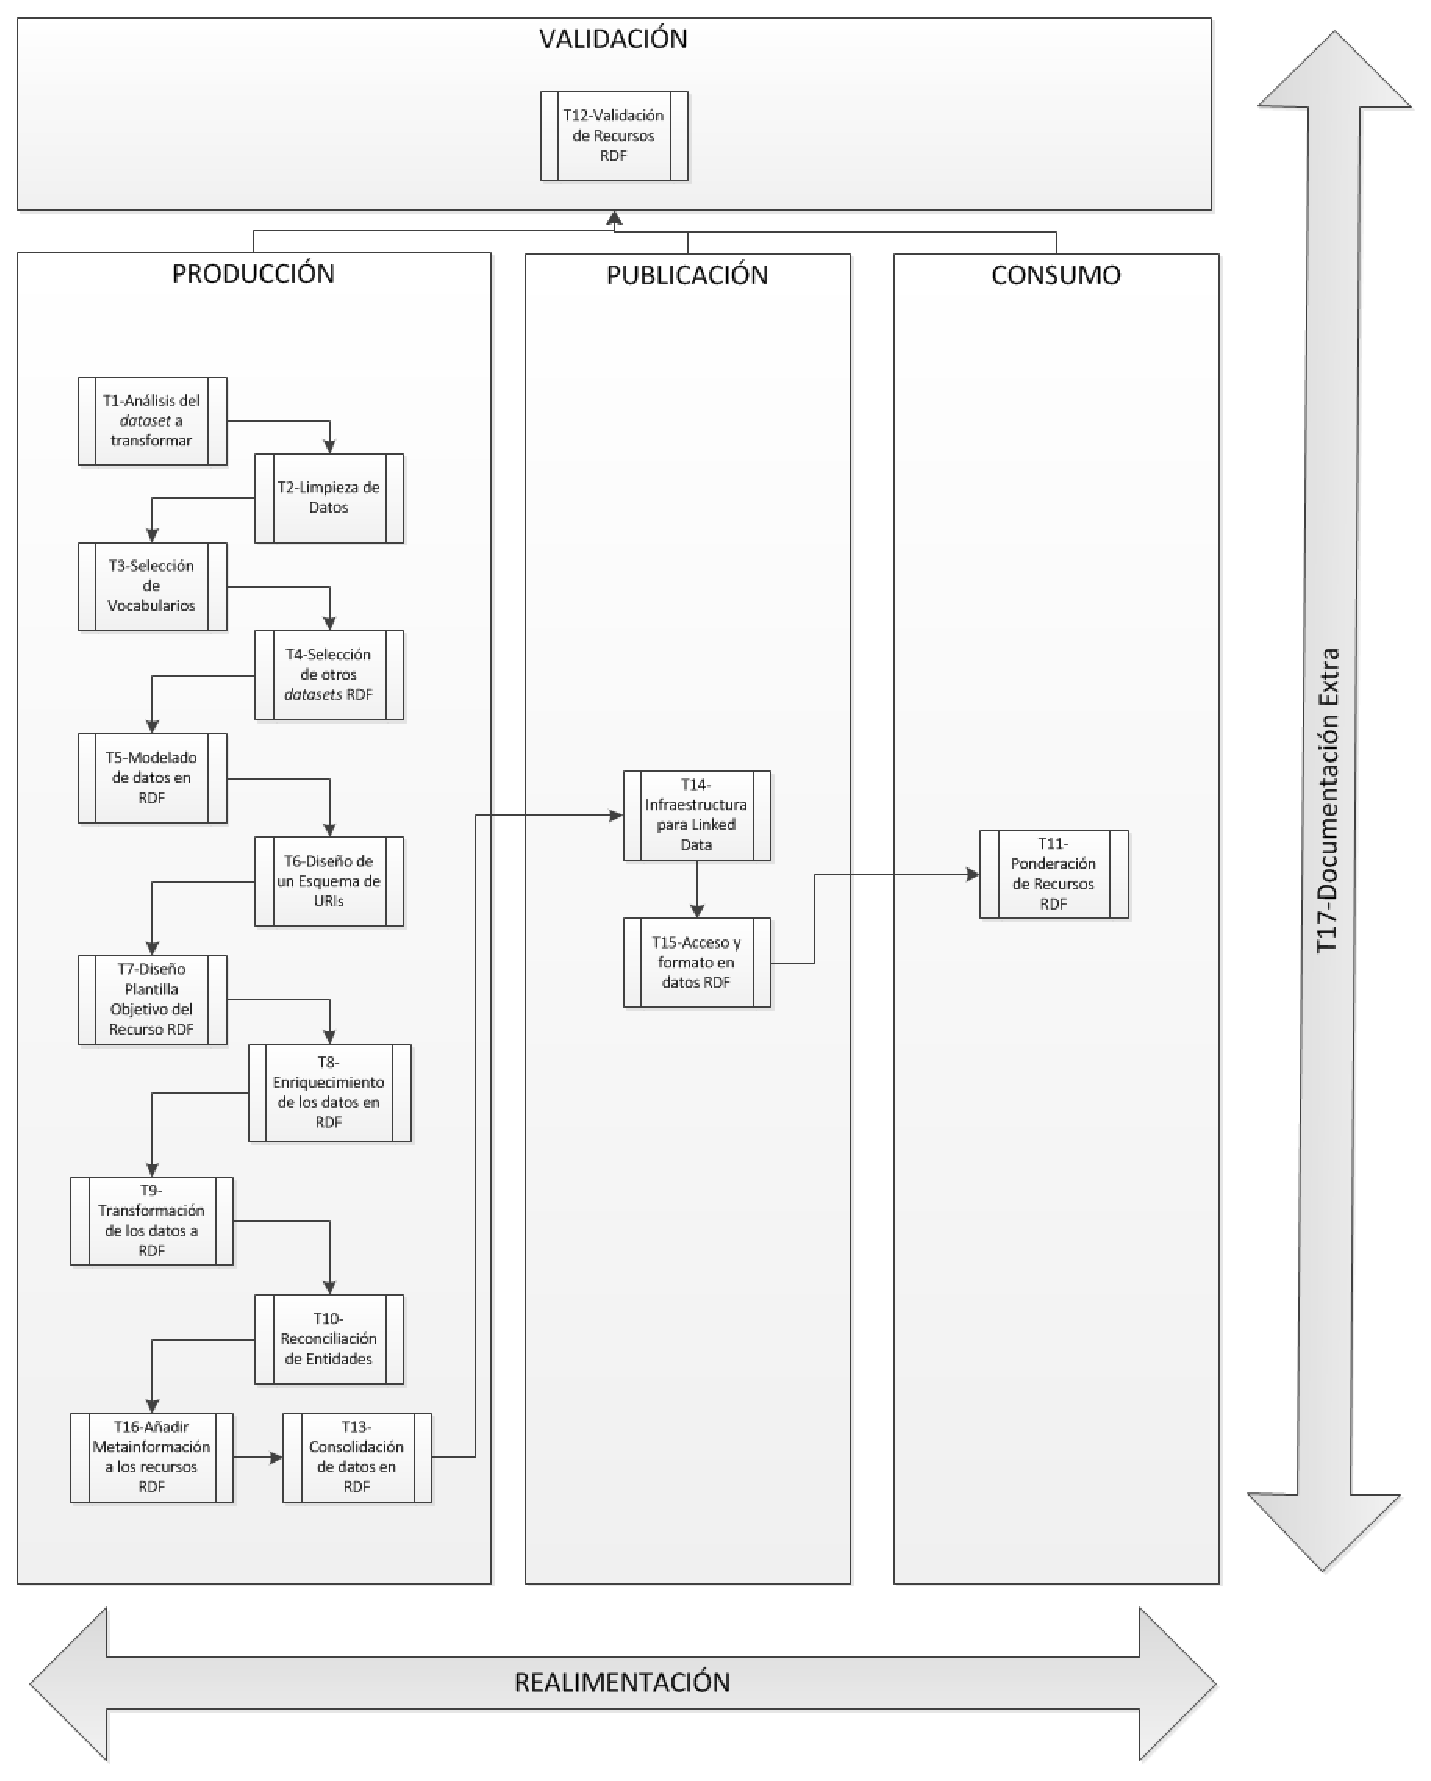
\includegraphics[width=5.8cm]{imgs/flujo-tareas}
% \end{figure}
% 
% }

\subsection*{Aplicación del Ciclo de Vida al e-Procurement}

\frame{
  \frametitle{Consideraciones Generales} 
\begin{block}{Procesos}<1->
 \begin{itemize}
 \item Métodos de Producción y Consumo dependiente del \dataset.
 \item Métodos de Publicación y Validación comunes.
\end{itemize}
\end{block}
\begin{exampleblock}{Conjuntos de Datos}<2->
\begin{itemize}
 \item Anuncios de licitación (PPN).
 \item Clasificaciones estándar de productos y servicios (PSCs).
 \item Organizaciones, personas y países.
\end{itemize} 
\end{exampleblock}

}


\frame{
  \frametitle{Métodos Aplicados} 
\begin{block}{Producción}<1->
Transformación de datos estáticos a RDF.
\end{block}
\begin{exampleblock}{Publicación}<2->
Fichero estático en RDF, \textit{Endpoint} de SPARQL y \linkeddata \textit{Frontend}.
\end{exampleblock}
\begin{alertblock}{Consumo}<3->
\textit{Mapeo} a Lenguaje de Programación.
\end{alertblock}
\begin{block}{Validación}<4->
Uso de Tablas de Validación.
\end{block}
\begin{exampleblock}{Realimentación}<5->
Actualización Ocasional.
\end{exampleblock}

}


% \frame{
%   \frametitle{Anuncios de Licitación} 
% \begin{figure}[htb]
% \centering
% 	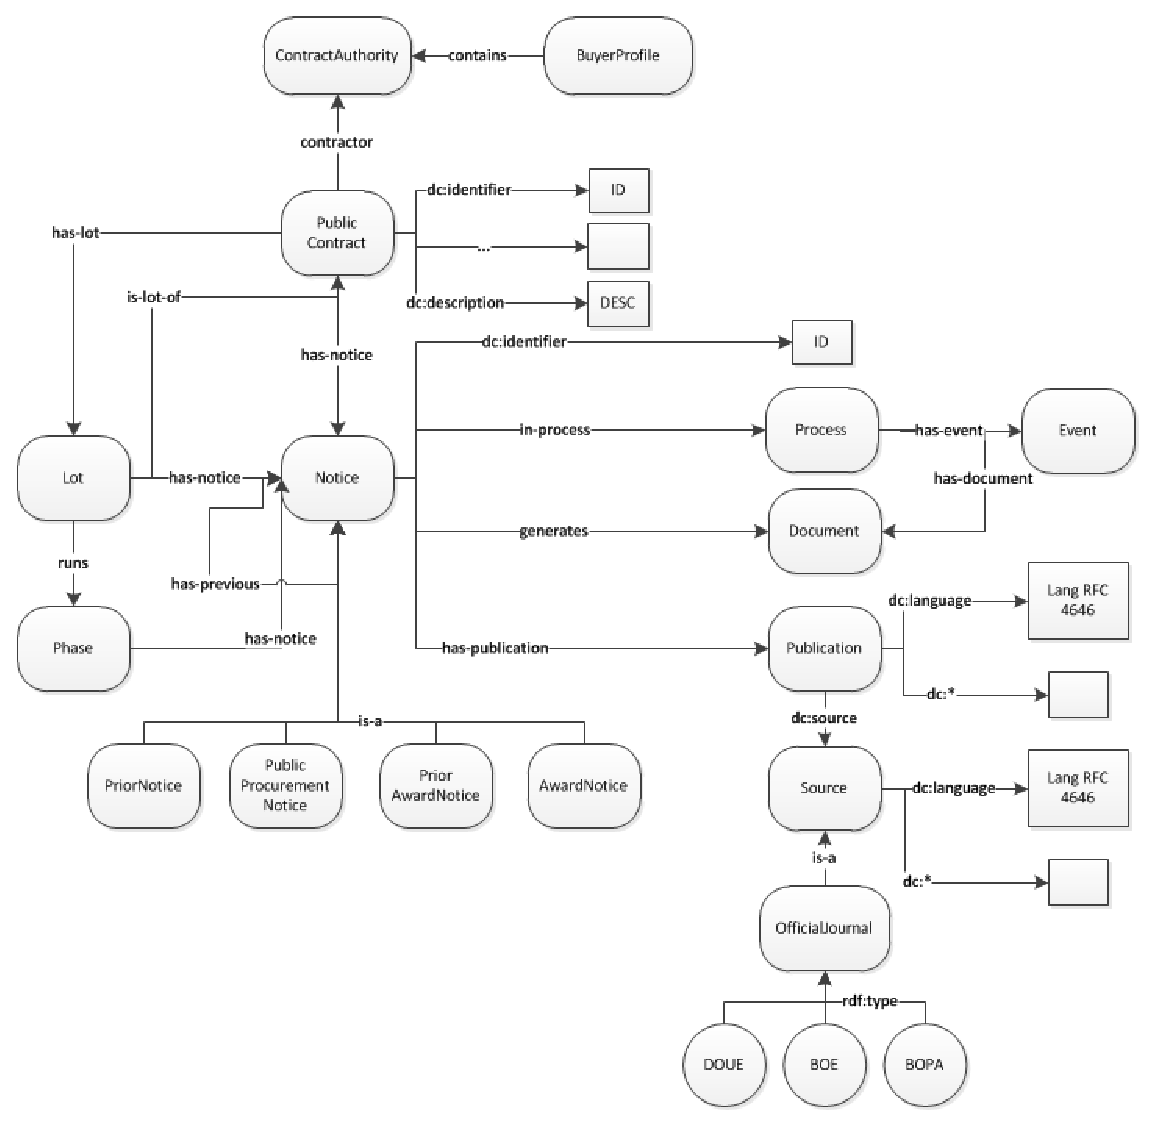
\includegraphics[width=6cm]{imgs/overview}
% \caption{Tarea $t_1$-Análisis del \dataset a transformar y Tarea $t_5$-Modelado de datos en RDF.}
% \end{figure}
% 
% }

% \frame{
%   \frametitle{Anuncios de Licitación} 
% \begin{figure}[htb]
% \centering
% 	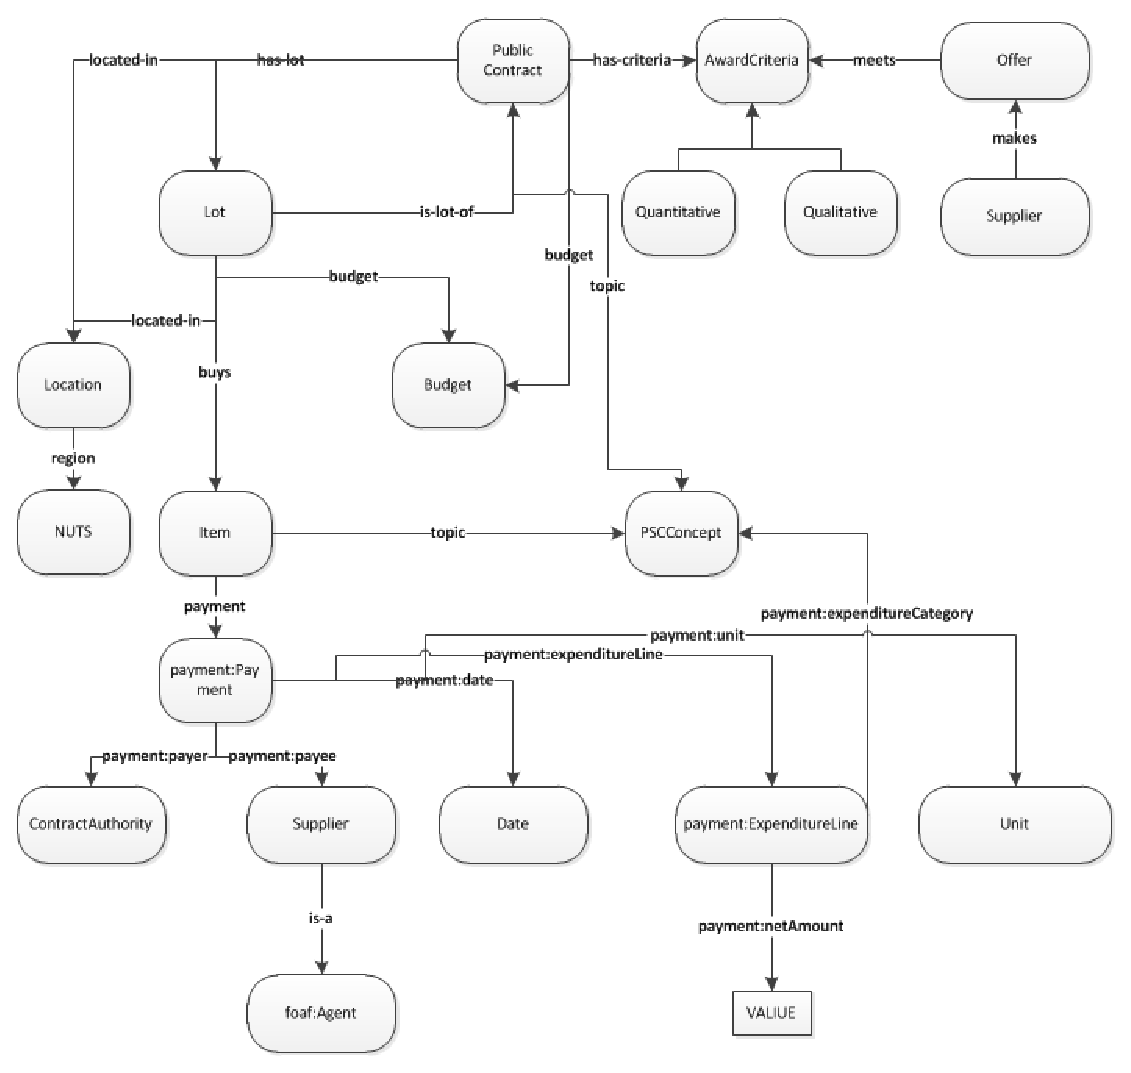
\includegraphics[width=6cm]{imgs/contract-lots}
% \caption{Tarea $t_1$-Análisis del \dataset a transformar y Tarea $t_5$-Modelado de datos en RDF (II).}
% \end{figure}
% 
% }

% \frame{
%   \frametitle{Anuncios de Licitación} 
% \begin{figure}[htb]
% \centering
% 	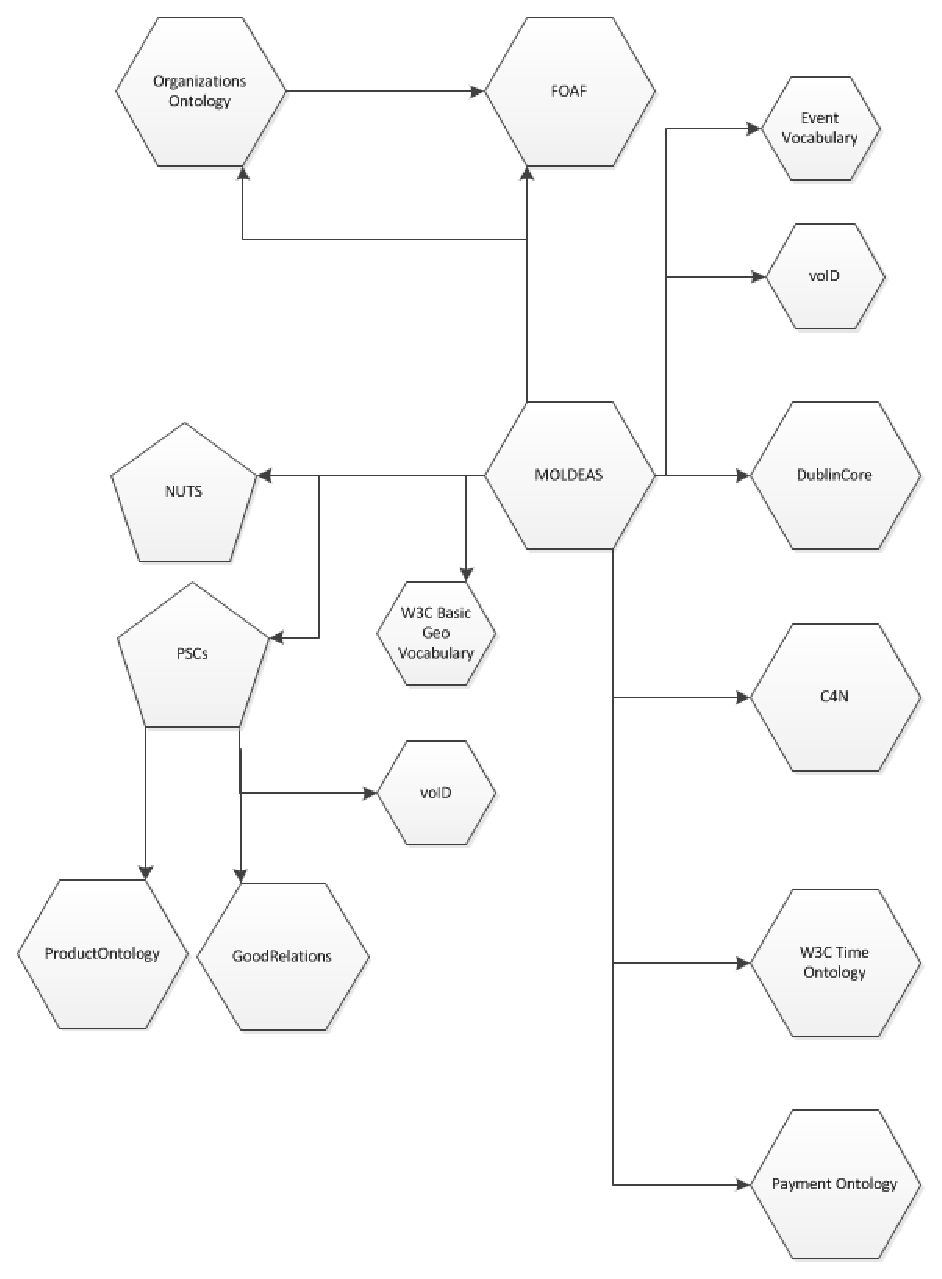
\includegraphics[width=4cm]{imgs/contract-vocabs}
% \caption{Tarea $t_3$-Selección de Vocabularios y Tarea $t_4$-Selección de otros \datasets RDF.}
% \end{figure}
% 
% }

% \frame{
%   \frametitle{Anuncios de Licitación} 
% \begin{figure}[htb]
% \centering
% 	\includegraphics[width=7cm]{imgs/t3}
% \caption{Tarea $t_3$-Selección de Vocabularios.}
% \end{figure}
% 
% }

% \frame{
%   \frametitle{Anuncios de Licitación} 
% \begin{figure}[htb]
% \centering
% 	\includegraphics[width=7cm]{imgs/t4}
% \caption{Tarea $t_4$-Selección de otros \datasets RDF.}
% \end{figure}
% 
% }

% \frame{
%   \frametitle{Anuncios de Licitación} 
% \begin{block}{$t_6$-Diseño de un Esquema de URIs.}
%  \begin{itemize}
% \item \url{http://purl.org/weso/ppn/} (<base\_uri>)
% \item \url{<base_uri>/ontology} 
% \item \url{<base_uri>/{year}} 
% \item \url{<base_uri>/resource/{year}/{id}}
% \item \url{<base_uri>/resource/{year}/{id}/publication/{id}}
% \item \url{<base_uri>/resource/{year}/{id}/lot/{id}} 
% \item \url{<base_uri>/resource/{year}/{id}/lot/{id}/item/{id}} 
% \item \url{<base_uri>/resource/{year}/{id}/lot/{id}/budget}
% \item \url{<base_uri>/resource/{year}/{id}/lot/{id}/payment}
% \item \ldots
% \end{itemize}  
% \end{block}
% 
% 
% }


\frame{
  \frametitle{Resultados} 
\small
\begin{longtable}[c]{|p{4cm}|p{3cm}|p{2cm}|} 
\hline
  \textbf{Anuncios de Licitación} & \textbf{Nº de Elementos}  &  \textbf{Tripletas}  \\\hline
\endhead
PPN 2008 & $112843$  &   $677058$  \\ \hline
PPN 2009 & $399766$ &   $2398601$   \\ \hline
PPN 2009  & $431813$&  $2590880$  \\ \hline
PPN 2011 & $67044$&   $402264$   \\ \hline
\multicolumn{3}{|c|}{\textbf{Catálogo de Anuncios de Licitación} (total)} \\ \hline
PPNs & $1011466$ &  $6068803$   \\ \hline
\hline
\end{longtable}

}


% \frame{
%   \frametitle{Anuncios de Licitación} 
% \begin{figure}[htb]
% \centering
% 	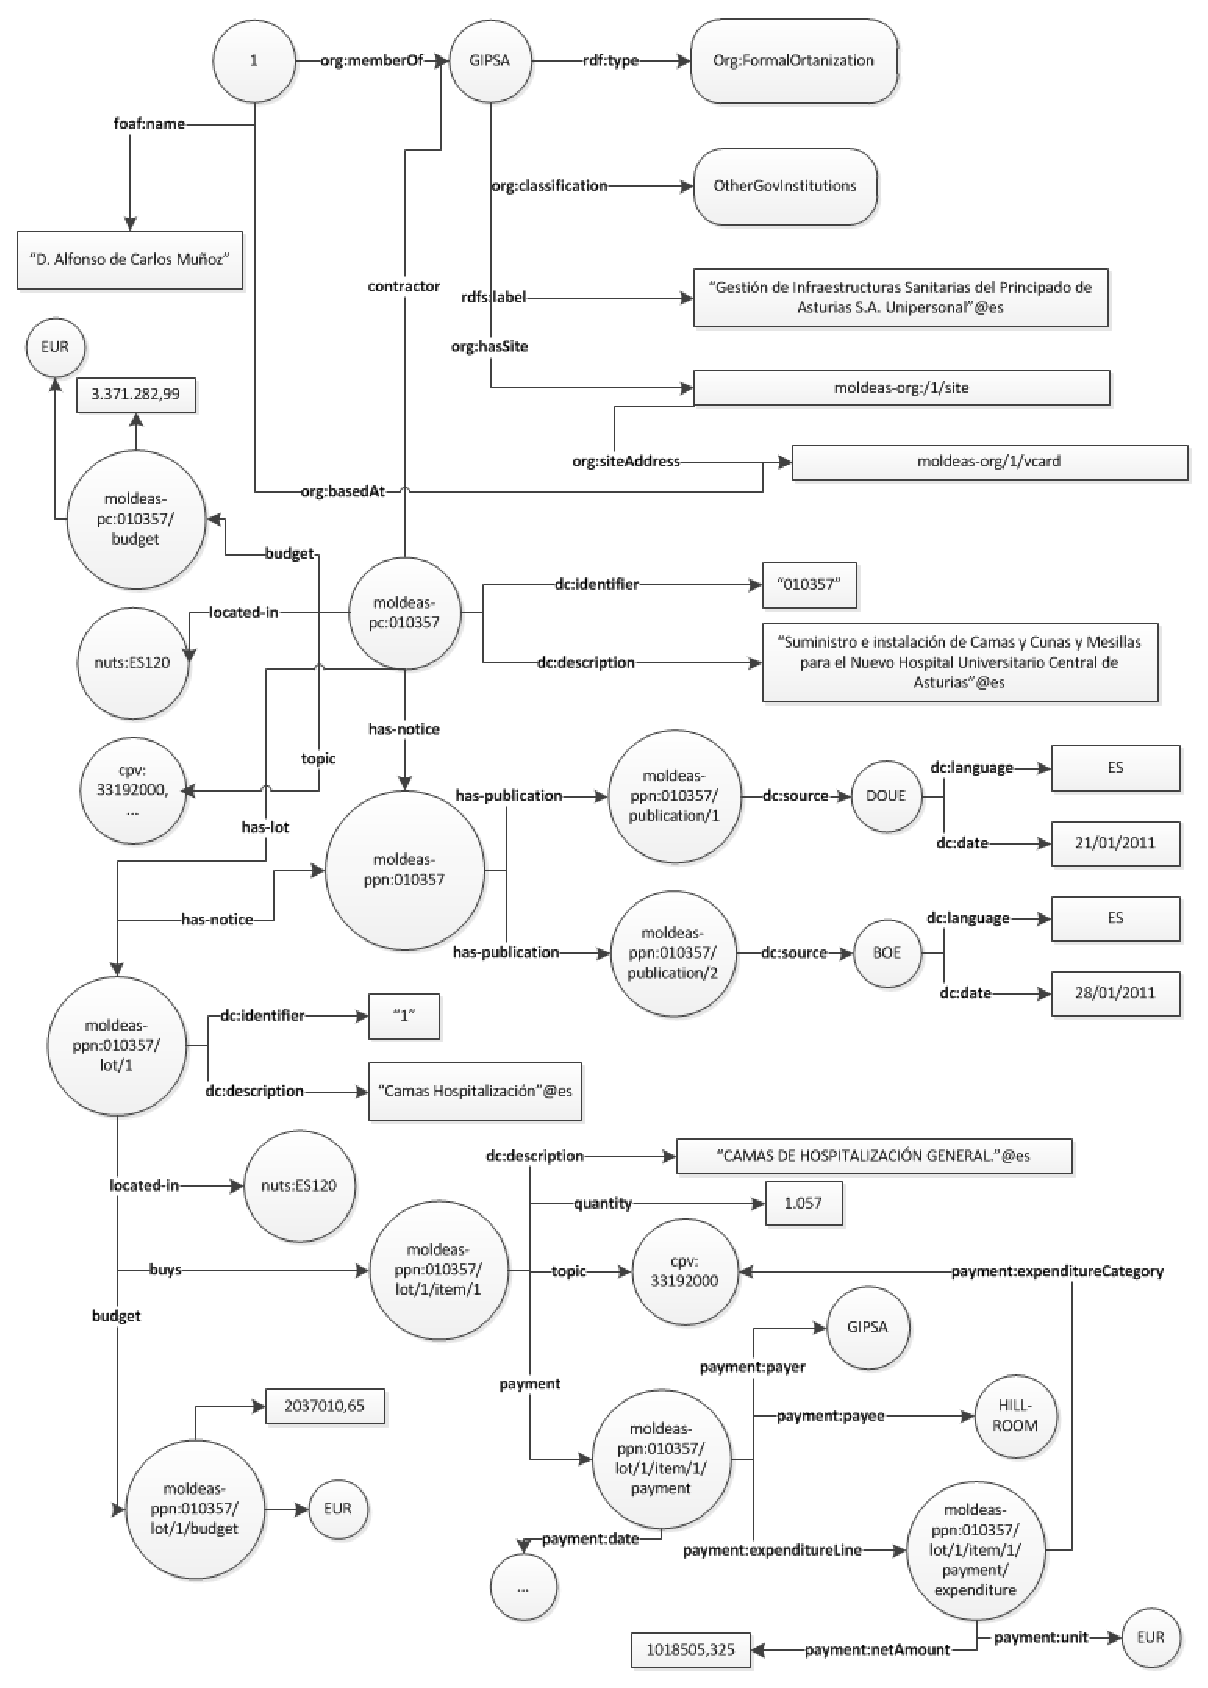
\includegraphics[width=5cm]{imgs/hospital-1}
% %\caption{Ejemplo licitación pública hospital.}
% \end{figure}
% 
% }

% \frame{
%   \frametitle{Anuncios de Licitación} 
% \begin{figure}[htb]
% \centering
% 	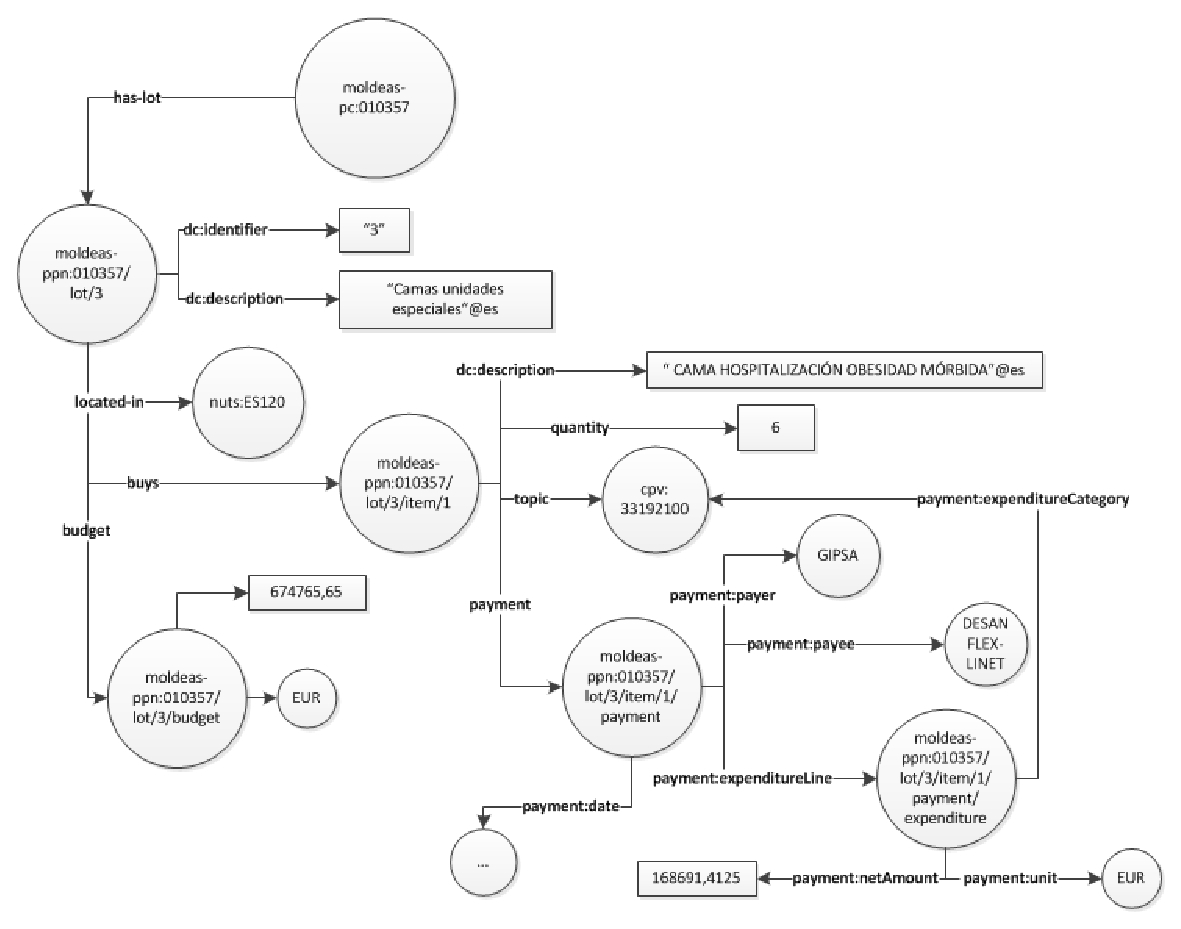
\includegraphics[width=9cm]{imgs/hospital-2}
% %\caption{Ejemplo licitación pública hospital.}
% \end{figure}
% 
% }


\frame{
  \frametitle{Clasificaciones Estándar de Productos y Servicios} 
\small
\begin{longtable}[c]{|p{6.5cm}|l|p{2cm}|} 
\hline
  \textbf{Clasificación} &  \textbf{Acrónimo} & \textbf{Organismo} \\\hline
\endhead
\textit{Common Procurement Vocabulary}, (2003 y 2008) & CPV & UE \\ \hline
\textit{Combined Nomenclature} 2012 (desde 1995) & CN & `` \\ \hline
\textit{Central Product Classification}, version 2 (2008) & CPC & \ldots\\ \hline
Clasificación de Productos por Actividad (2008) & CPA & `` \\ \hline
\textit{International Standard Industrial Classification of All Economic Activities, Rev.4} & ISIC & ONU \\ \hline
\textit{North American Industry Classification System} 2007 y 2012 & NAICS & EEUU \\ \hline
\textit{Standard International Trade Classification, Revision 4} & SITC & ONU \\ \hline
\hline
\end{longtable}

}

% \frame{
%   \frametitle{Clasificaciones Estándar de Productos y Servicios} 
% 
% \begin{enumerate}
%  \item Categorías de productos.  $Cat_{psc} = \displaystyle\bigcup_{n=0}^k{(Cat_{psc}^n)}$
% \begin{itemize}
%  \item Organización jerárquica: $Cat_{psc}^0\succ
% Cat_{psc}^1\succ...\succ Cat_{psc}^n $.
%  \item Cada elemento $t_{psc}^x$ pertenece a una, y sólo una, categoría de productos.
%   \item Categorías disjuntas: $\displaystyle\bigcap_{n=0}^k{(Cat_{psc}^n)}=\emptyset$.
% \end{itemize}
% 
% \item  Estructura taxonómica.  Cada sector es un árbol, $T_{psc}$: todos los elementos
% $t_{psc}^n$ tienen un elemento de nivel superior $t_{psc}^{n-1}$. El conjunto de sectores puede definirse como 
% un \textbf{bosque} ($\mathbb{F}_{psc}$) de árboles ($T_{psc}$):
% \begin{itemize}
%  \item $\mathbb{F}_{psc}= \displaystyle\bigcup_{m=0}^k{(T_{psc}^m)}$, con raíz $t_{psc}^0$.
%  \item Cada elemento $t_{psc}$ pertenece a uno de estos árboles de productos $T_{psc}^x$.
% \end{itemize}
%  
% \end{enumerate}
% 
% 
% }

% \frame{
%   \frametitle{Clasificaciones Estándar de Productos y Servicios} 
% \begin{figure}[htb]
% \centering
% 	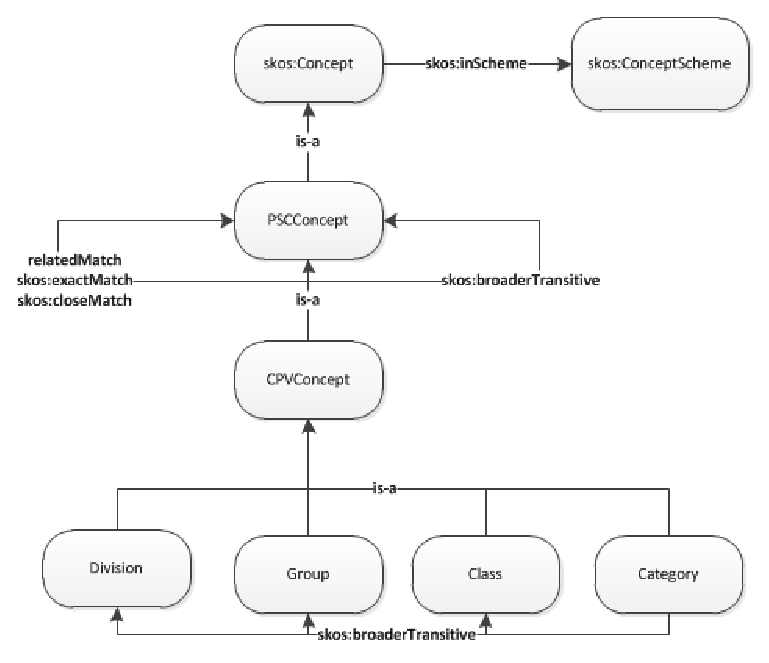
\includegraphics[width=6cm]{imgs/pscs-model}
% \caption{Tarea $t_1$-Análisis del \dataset a transformar y Tarea $t_5$-Modelado de datos en RDF.}
% \end{figure}
% 
% }

\frame{
  \frametitle{Clasificaciones Estándar de Productos y Servicios} 
\begin{figure}[!htb]
\centering
	\includegraphics[width=12cm]{./imgs/pscs}
\caption{Enlaces entre las distintas Clasificaciones Estándar de Productos y Servicios.}
\end{figure}
}

% 
% \frame{
%   \frametitle{Clasificaciones Estándar de Productos y Servicios} 
% \begin{block}{$t_6$-Diseño de un Esquema de URIs.}
%  \begin{itemize}
% \item \url{http://purl.org/weso/pscs/}
% \item \url{<base_uri>/ontology}
% \item \url{<base_uri>/resource/ds}
% \item \url{<base_uri>/{psc}/{version|year}}
% \item \url{<base_uri>/{psc}/{version|year}/ontology} 
% \item \url{<base_uri>/resource/{psc}/{version|year}/{id}} 
% \item \url{<base_uri>/resource/{psc}/{version|year}/ds} 
% \end{itemize}  
% \end{block}
% 
% 
% }


\frame{
  \frametitle{Resultados-I} 
\small
\begin{longtable}[c]{|l|p{1.5cm}|p{1.8cm}|p{1.5cm}|p{2.5cm}|} 
\hline
  \textbf{PSC} & \textbf{\#}  &  \textbf{Tripletas} &  \textbf{Links} &  \textbf{Links CPV 2008} \\\hline
\endhead
CPV 2003 & $8323$  & $546135$  & $8322$ & $462$ (del CPV 2008 al 2003)   \\ \hline
CPV 2008 & $10357$ &   $803311$  & $10355$ & N/A   \\ \hline
CN 2012  & $14552$&  $137484$  & $2590$ & $2390$ \\ \hline
CPC 2008 & $4408$&   $100819$  & $4408$ & $4375$ y $1503$ (exactos)  \\ \hline
CPA 2008 & $5429$&  $92749$   & $5429$ & $5399$  \\ \hline
\multicolumn{5}{|c|}{\ldots} \\ \hline
\hline
\end{longtable}

}


\frame{
  \frametitle{Resultados-II} 
\small
\begin{longtable}[c]{|l|p{1.5cm}|p{1.8cm}|p{1.5cm}|p{2.5cm}|} 
\hline
  \textbf{PSC} & \textbf{\#}  &  \textbf{Tripletas} &  \textbf{Links} &  \textbf{Links CPV 2008} \\\hline
\endhead
ISIC v4  & $766$&  $18986$   & $766$ & $765$  \\ \hline
NAICS 2007 & $2328$&  $36292$   & $2328$ & $2300$  \\ \hline
NAICS 2012 & $2212$&  $35390$   & $2212$ & $2186$  \\ \hline
SITC v4 & $4017$&  $70887$   & $3941$ & $3811$  \\ \hline
\multicolumn{5}{|c|}{\textbf{Catálogo de Clasificaciones Estándar de Productos} (total)} \\ \hline
PSCs & $52392$ &   $1842053$ & $40351$ & $23191$  \\ \hline
\hline
\end{longtable}

}

\frame{
  \frametitle{Organizaciones, personas y países} 

\begin{figure}[htb]
\centering
	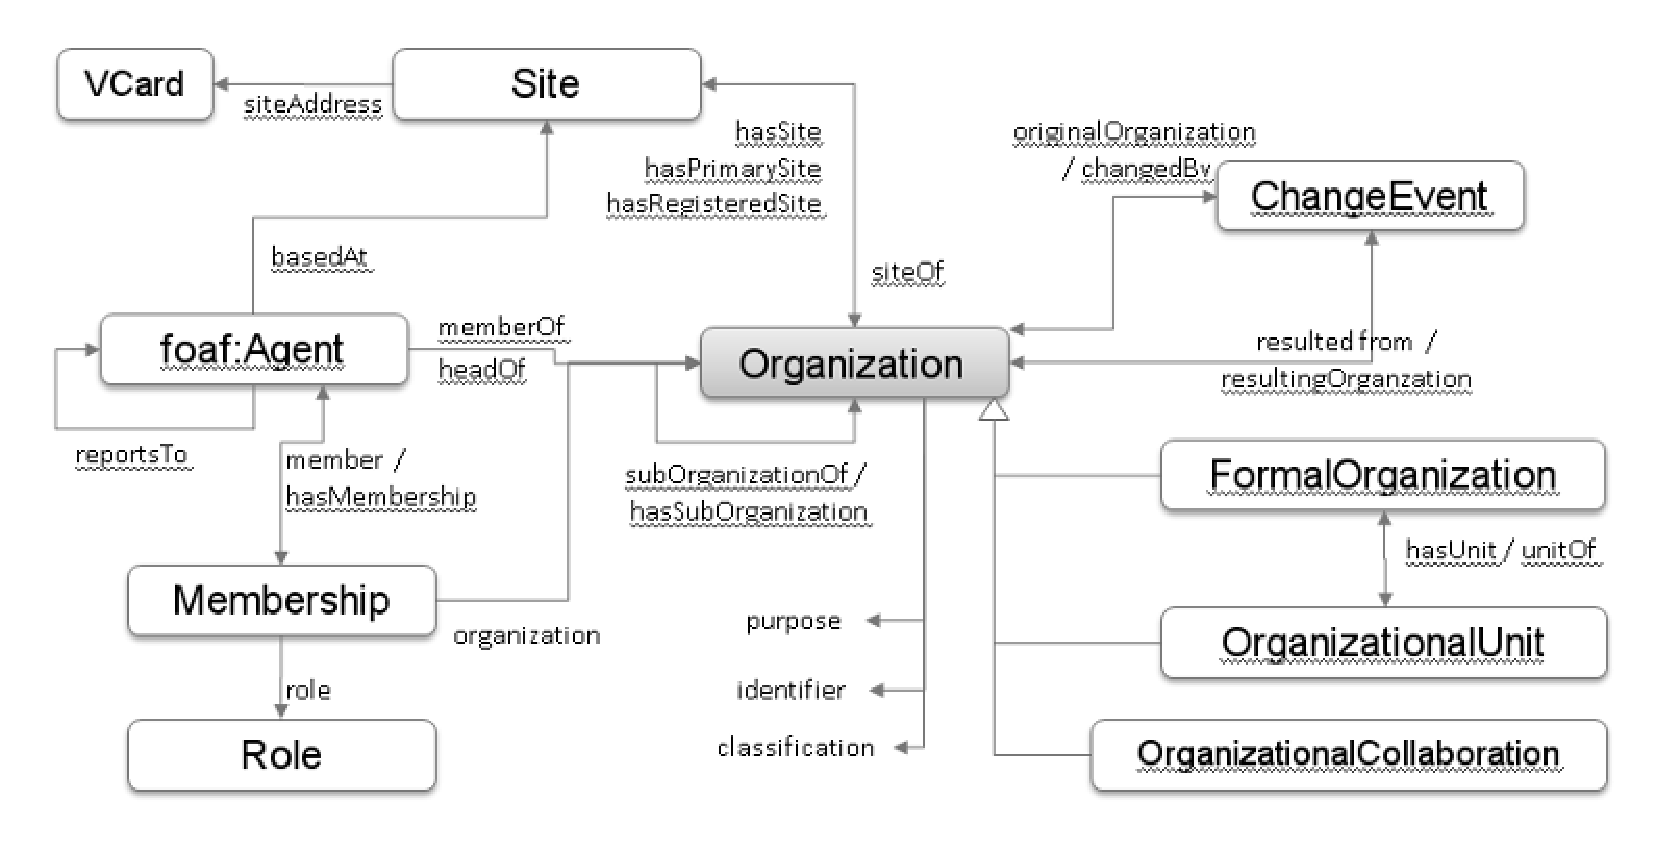
\includegraphics[width=8cm]{imgs/org}
\caption{\textit{Organizations Ontology} del W3C.}
\end{figure}

}

% \frame{
%   \frametitle{Organizaciones, personas y países} 
% \begin{block}{$t_6$-Diseño de un Esquema de URIs.}
%  \begin{itemize}
% \item \url{http://purl.org/weso/eprocurement}
% \item \url{<base_uri>/organization/ontology}
% \item \url{<base_uri>/organization/resource/ds} 
% \item \url{<base_uri>/organization/resource/{id}} 
% \item \url{<base_uri>/organization/person/resource/ds}
% \item \url{<base_uri>/organization/person/resource/{id}}
% \item \url{<base_uri>/country/ontology}
% \item \url{<base_uri>/country/resource/ds} 
% \item \url{<base_uri>/country/resource/{id}}
% \end{itemize}  
% \end{block}
% }


\frame{
  \frametitle{Resultados} 
\small
\begin{longtable}[c]{|p{2.2cm}|p{2.5cm}|p{2cm}|p{2.5cm}|} 
\hline
  \textbf{Dataset} & \textbf{\#}  &  \textbf{Tripletas} &  \textbf{Enlaces externos}  \\\hline
\endhead
Organizaciones & $50000$   & $1150020$  & $50000$ (países)   \\ \hline
Personas & $50000$    & $900219$  & $50000$  (países)  \\ \hline
Países & $246$     & $1756$  & $1779$ \\ \hline
\multicolumn{4}{|c|}{\textbf{Organizaciones, Personas y Países} (total)} \\ \hline
Agregado & $100246$  & $2051995$ & $101779$   \\ \hline
\hline
\end{longtable}

}


% \frame{
%   \frametitle{Tareas Transversales} 
% \begin{block}{Tarea $t_{12}$-Validación de Recursos RDF}
%  \begin{itemize}
%  \item Los datos RDF son correctos, ya que se ha utilizado el API de Jena.
%  \item El dominio y rango en las propiedades es correcta, la validación contra el modelo definido.
%  \item Se ha establecido metainformación sobre la procedencia a nivel de \dataset.
%  \item Todos los recursos transformados siguen la plantilla objetivo RDF.
% \end{itemize}
% \end{block}
% 
% 
% }

% \frame{
%   \frametitle{Tareas Transversales} 
% \begin{figure}[htb]
% \centering
% 	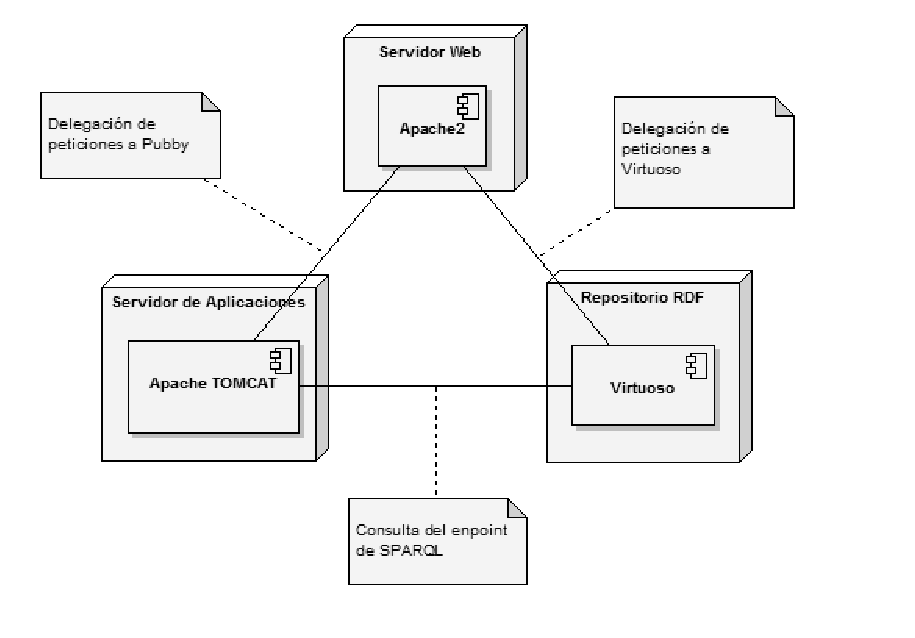
\includegraphics[width=8cm]{imgs/infra-ld}
% \caption{Tarea $t_{14}$-Infraestructura para \linkeddata.}
% \end{figure}
% 
% }

% \frame{
%   \frametitle{Tareas Transversales} 
% \small
% \begin{table}[!htb]
% \renewcommand{\arraystretch}{1.3}
% \begin{center}
% \begin{tabular}{|p{4cm}|l|p{4cm}|}
% \hline
%   \textbf{Acceso} &  \textbf{Formato} &  \textbf{Provisto por}  \\\hline
%  Petición GET    & N3/Turtle    & Apache2 \\ \hline
%  Consulta SPARQL & \textit{Spreadsheet}  & \textit{Endpoint} de SPARQL  \\ \hline
%  ``       & XML 		& ``\\ \hline
%  ``       & JSON 	& ``\\ \hline
%  ``       & Javascript 	& `` \\ \hline 
%  Consulta SPARQL y petición GET & N3/Turtle 	& \textit{Endpoint} de SPARQL y \linkeddata \textit{Frontend} \\ \hline
%  ``       & RDF/XML 	& ``\\ \hline
%  ``       & NTriples 	& `` \\ \hline
%  ``       & HTML 	& `` \\ \hline
%  \hline
%   \end{tabular}
%   \end{center}
% \caption{Tarea $t_{15}$-Acceso y formato en datos RDF.}
% \end{table} 
% }

% \frame{
%   \frametitle{Tareas Transversales} 
% \begin{block}{Tareas}
%  \begin{itemize}
%  \item $t_2$-Limpieza de datos (N/A).
%  \item $t_7$-Diseño Plantilla Objetivo del Recurso RDF (dependiente del contexto).
%  \item $t_8$-Enriquecimiento de los datos en RDF (\``).
%  \item $t_9$-Transformación de los datos a RDF.
%  \item $t_{10}$-Reconciliación de Entidades.
%  \item $t_{11}$-Ponderación de Recursos RDF.
%  \item $t_{13}$-Consolidación de datos RDF (N/A).
%  \item $t_{16}$-Añadir metainformación a los recursos RDF (\textit{voID}).
%  \item $t_{17}$-Documentación extra.
% \end{itemize}
% \end{block}
% }

\subsection*{Sistema MOLDEAS}


\frame{
  \frametitle{MOLDEAS y los procesos del Ciclo de Vida} 

\begin{figure}[htb]
\centering
	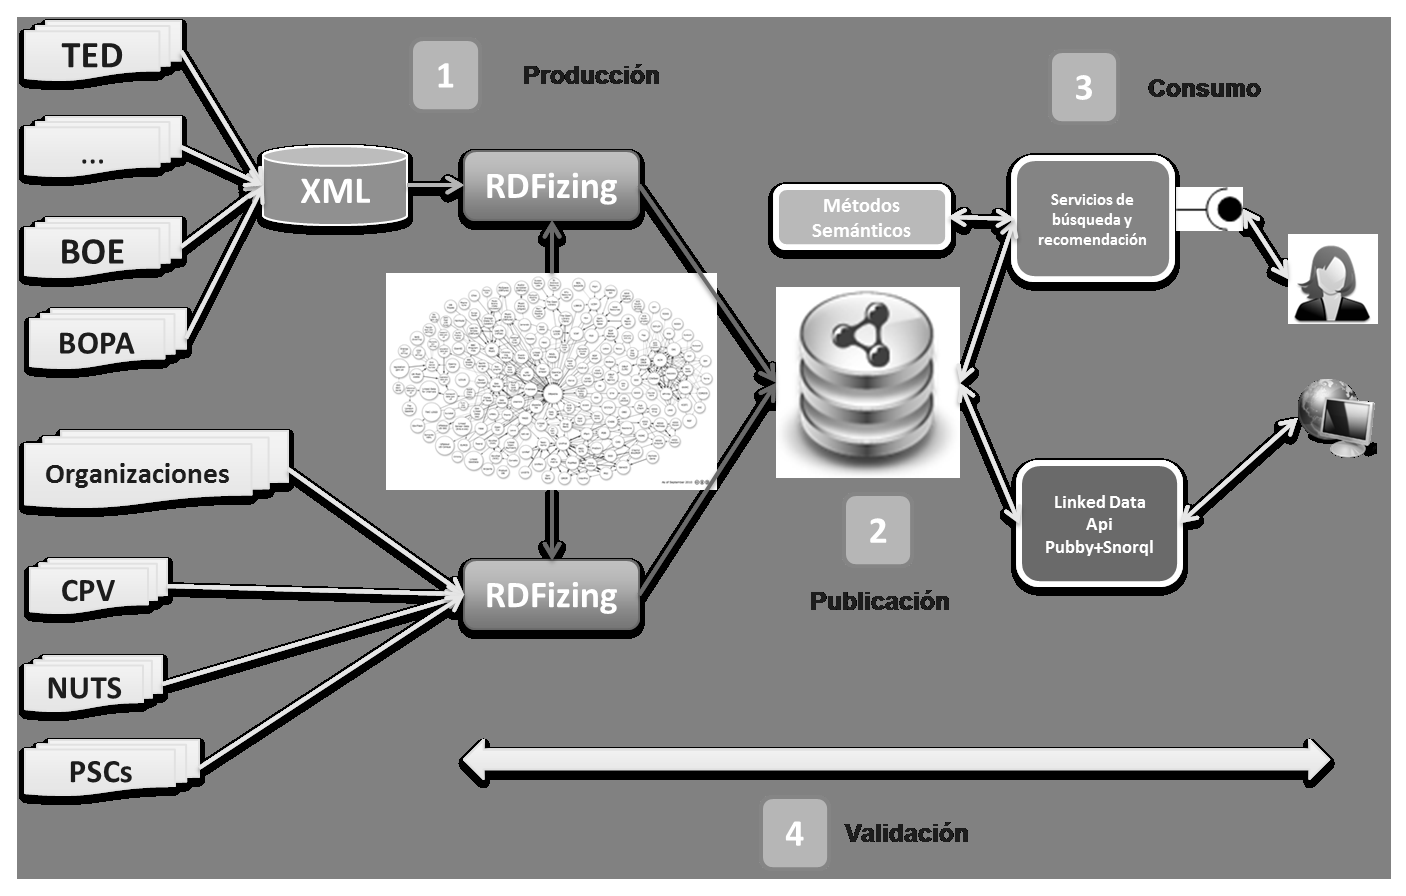
\includegraphics[width=8cm]{imgs/functional-overview}
\caption{Visión Funcional de MOLDEAS y los procesos del Ciclo de Vida de \linkeddata.}
\end{figure}
}

% \frame{
%   \frametitle{Consideraciones de Diseño} 
% \begin{block}{Buenas Prácticas}
%  \begin{itemize}
%  \item Uso de patrones de diseño: \textit{DAO, Chain of Responsibility, Adapter, TransferObject}, etc.
%  \item Aplicación por capas (Datos, Servicios, Cliente y Presentación).
%  \item Reutilización de bibliotecas existentes.
% \end{itemize}
% \end{block}
% }


% \frame{
%   \frametitle{Componentes MOLDEAS} 
% \begin{figure}[!htb]
% \centering
% 	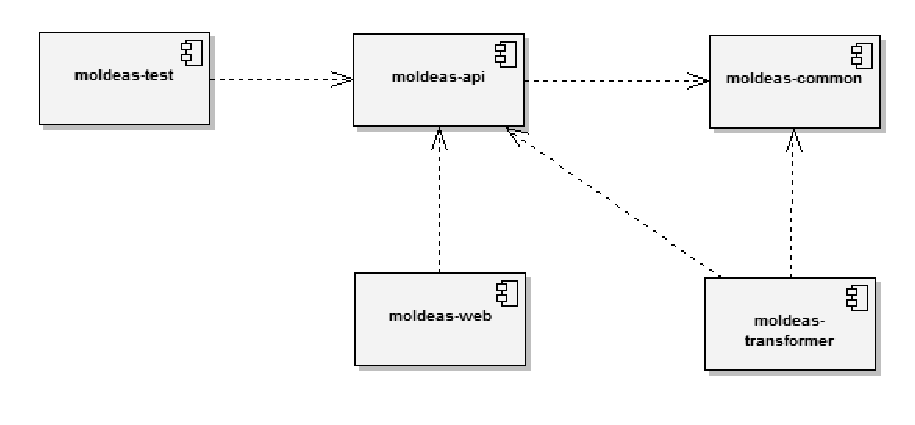
\includegraphics[width=8cm]{imgs/moldeas-componentes}
% \caption{Dependencias entre componentes en el sistema MOLDEAS.}
% \end{figure}
% }

% \frame{
%   \frametitle{Arquitectura General} 
% \begin{figure}[!htb]
% \centering
% 	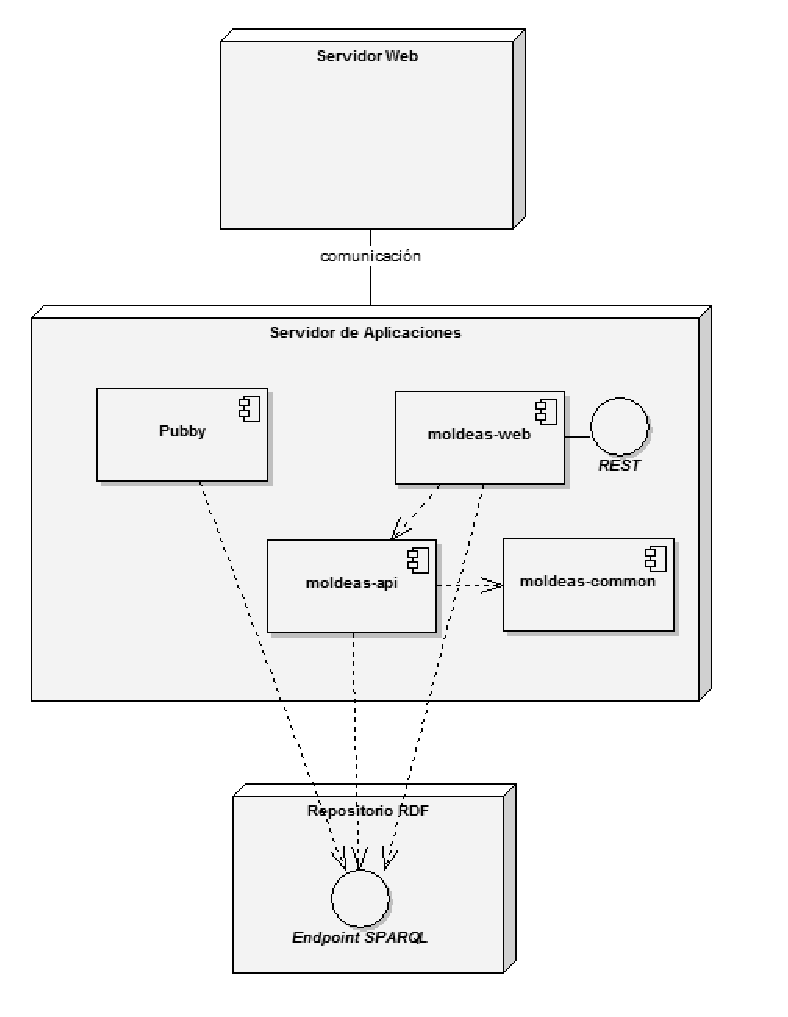
\includegraphics[width=5cm]{imgs/moldeas-despliegue}
% \caption{Diagrama de Despliegue.}
% \end{figure}
% 
% }


% \frame{
%   \frametitle{Entorno Tecnológico} 
% 
% 
% \begin{columns}[c] % the \ldotsc\ldots option specifies center vertical alignment
% \column{.5\textwidth} % column designated by a command
% 
% 
% \begin{block}{Desarrollo}<1->
%  \begin{itemize}
% \item Java 1.6.
% \item Apache Maven2.
% \item Eclipse-IDE.
% \item Repositorio Google Code.
% \item Protégé 4.1.x.
% \item Openlink Virtuoso 6.1.
% \item Google Refine y \textit{RDF extension}.
% \item \LaTeX.
% \end{itemize}
% \end{block}
% 
% 
% \column{.5\textwidth}
% 
% \begin{exampleblock}{Bibliotecas destacadas}<2->
%  \begin{itemize}
% \item Log4j 1.2.14.
% \item Junit 4.0.
% \item Apache Lucene 2.9.0.
% \item Apache Solr 1.4.1.
% \item Apache Mahout 0.4.
% \item Spring 2.5
% \item Jersey-REST 0.8.
% \item Jquery 1.4.1.
% \item Exhibit 2.2.0.
% \item Pubby 0.3.3.
% \item SNORQL.
% \end{itemize}
% \end{exampleblock}
% 
% \end{columns}
% 
% 
% }

% \frame{
%   \frametitle{Componentes: moldeas-api} 
% \begin{figure}[!htb]
% \centering
%  \includegraphics[width=9cm]{imgs/query-expansion}
% \caption{Métodos de Expansión de Consulta.}
% \end{figure}
% }
% 
% \frame{
%   \frametitle{Pruebas y Validación} 
% \begin{exampleblock}{Pruebas de Código Fuente}
%  \begin{itemize}
%  \item $140$ \textit{tests}.
%  \item $48$ clases Java específicas para Junit.
%  \item Métricas de código fuente de alta cohesión y bajo acoplamiento.
% \end{itemize}
% \end{exampleblock}
% }

\frame{
  \frametitle{MOLDEAS web (REST+Jquery)} 
\begin{figure}[!htb]
\centering
	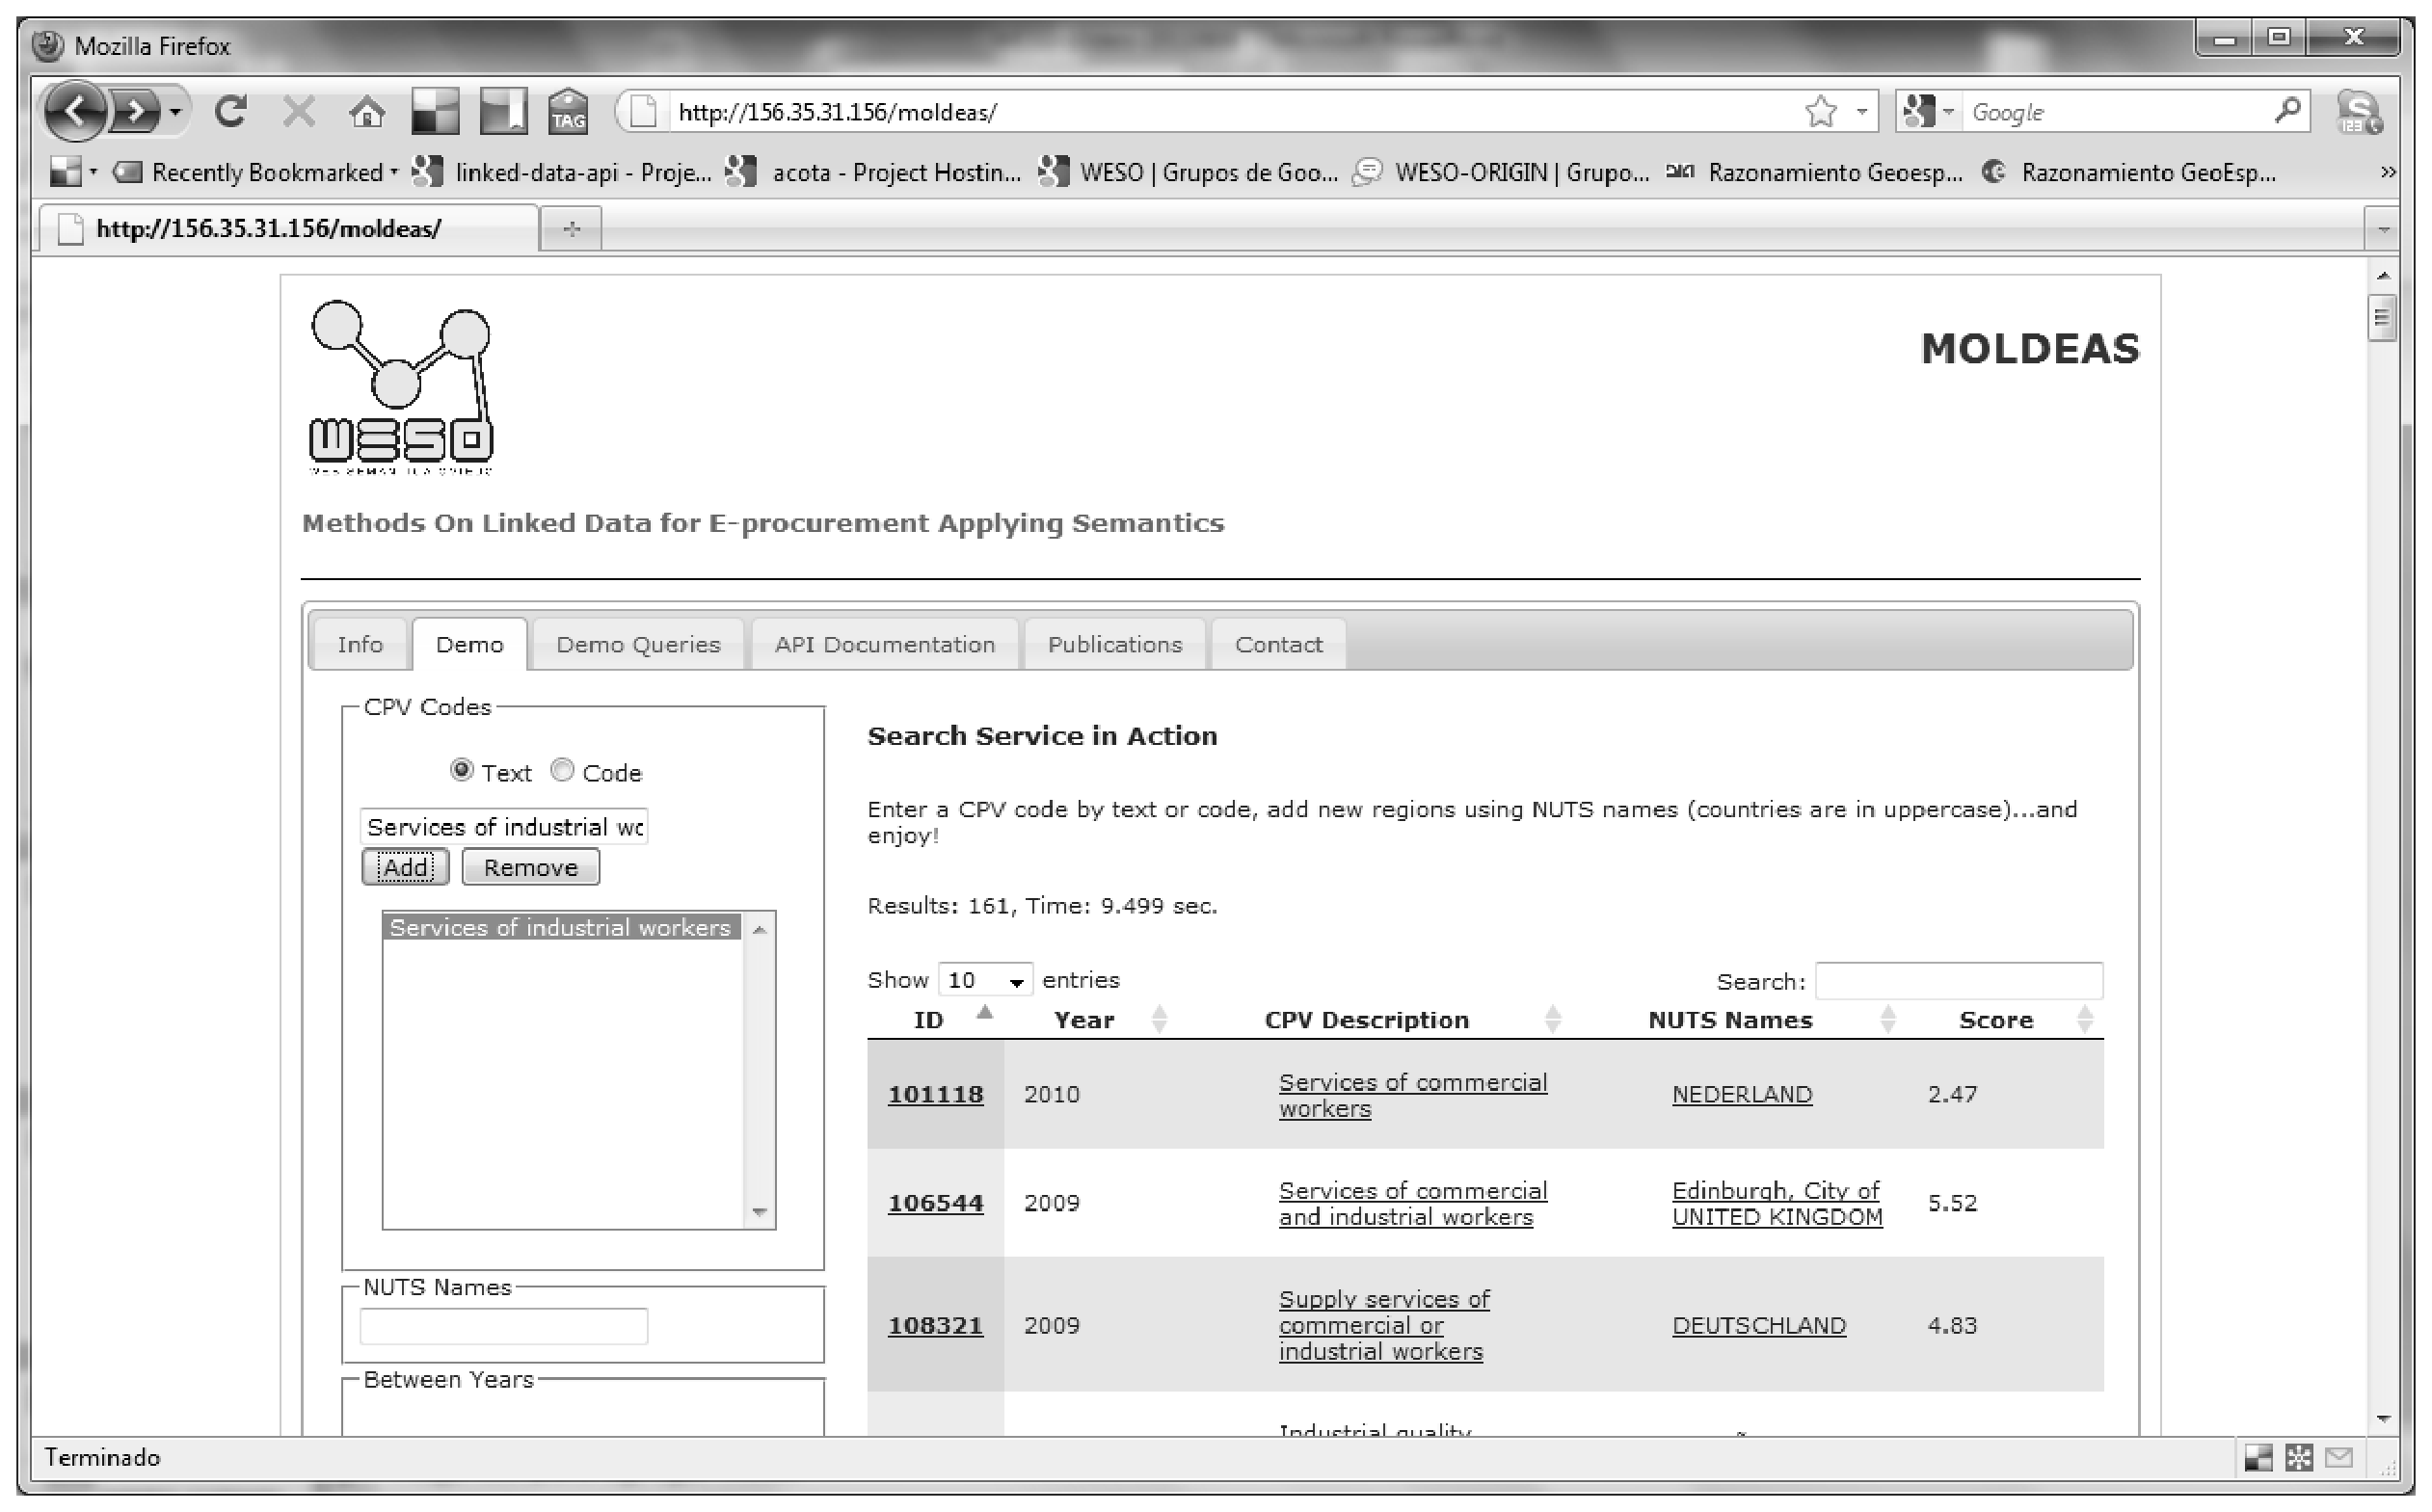
\includegraphics[width=10cm]{imgs/moldeas-web}
\end{figure}

}
\frame{
  \frametitle{MOLDEAS web-Resultados (Jquery+Exhibit)} 
\begin{figure}[!htb]
\centering
 	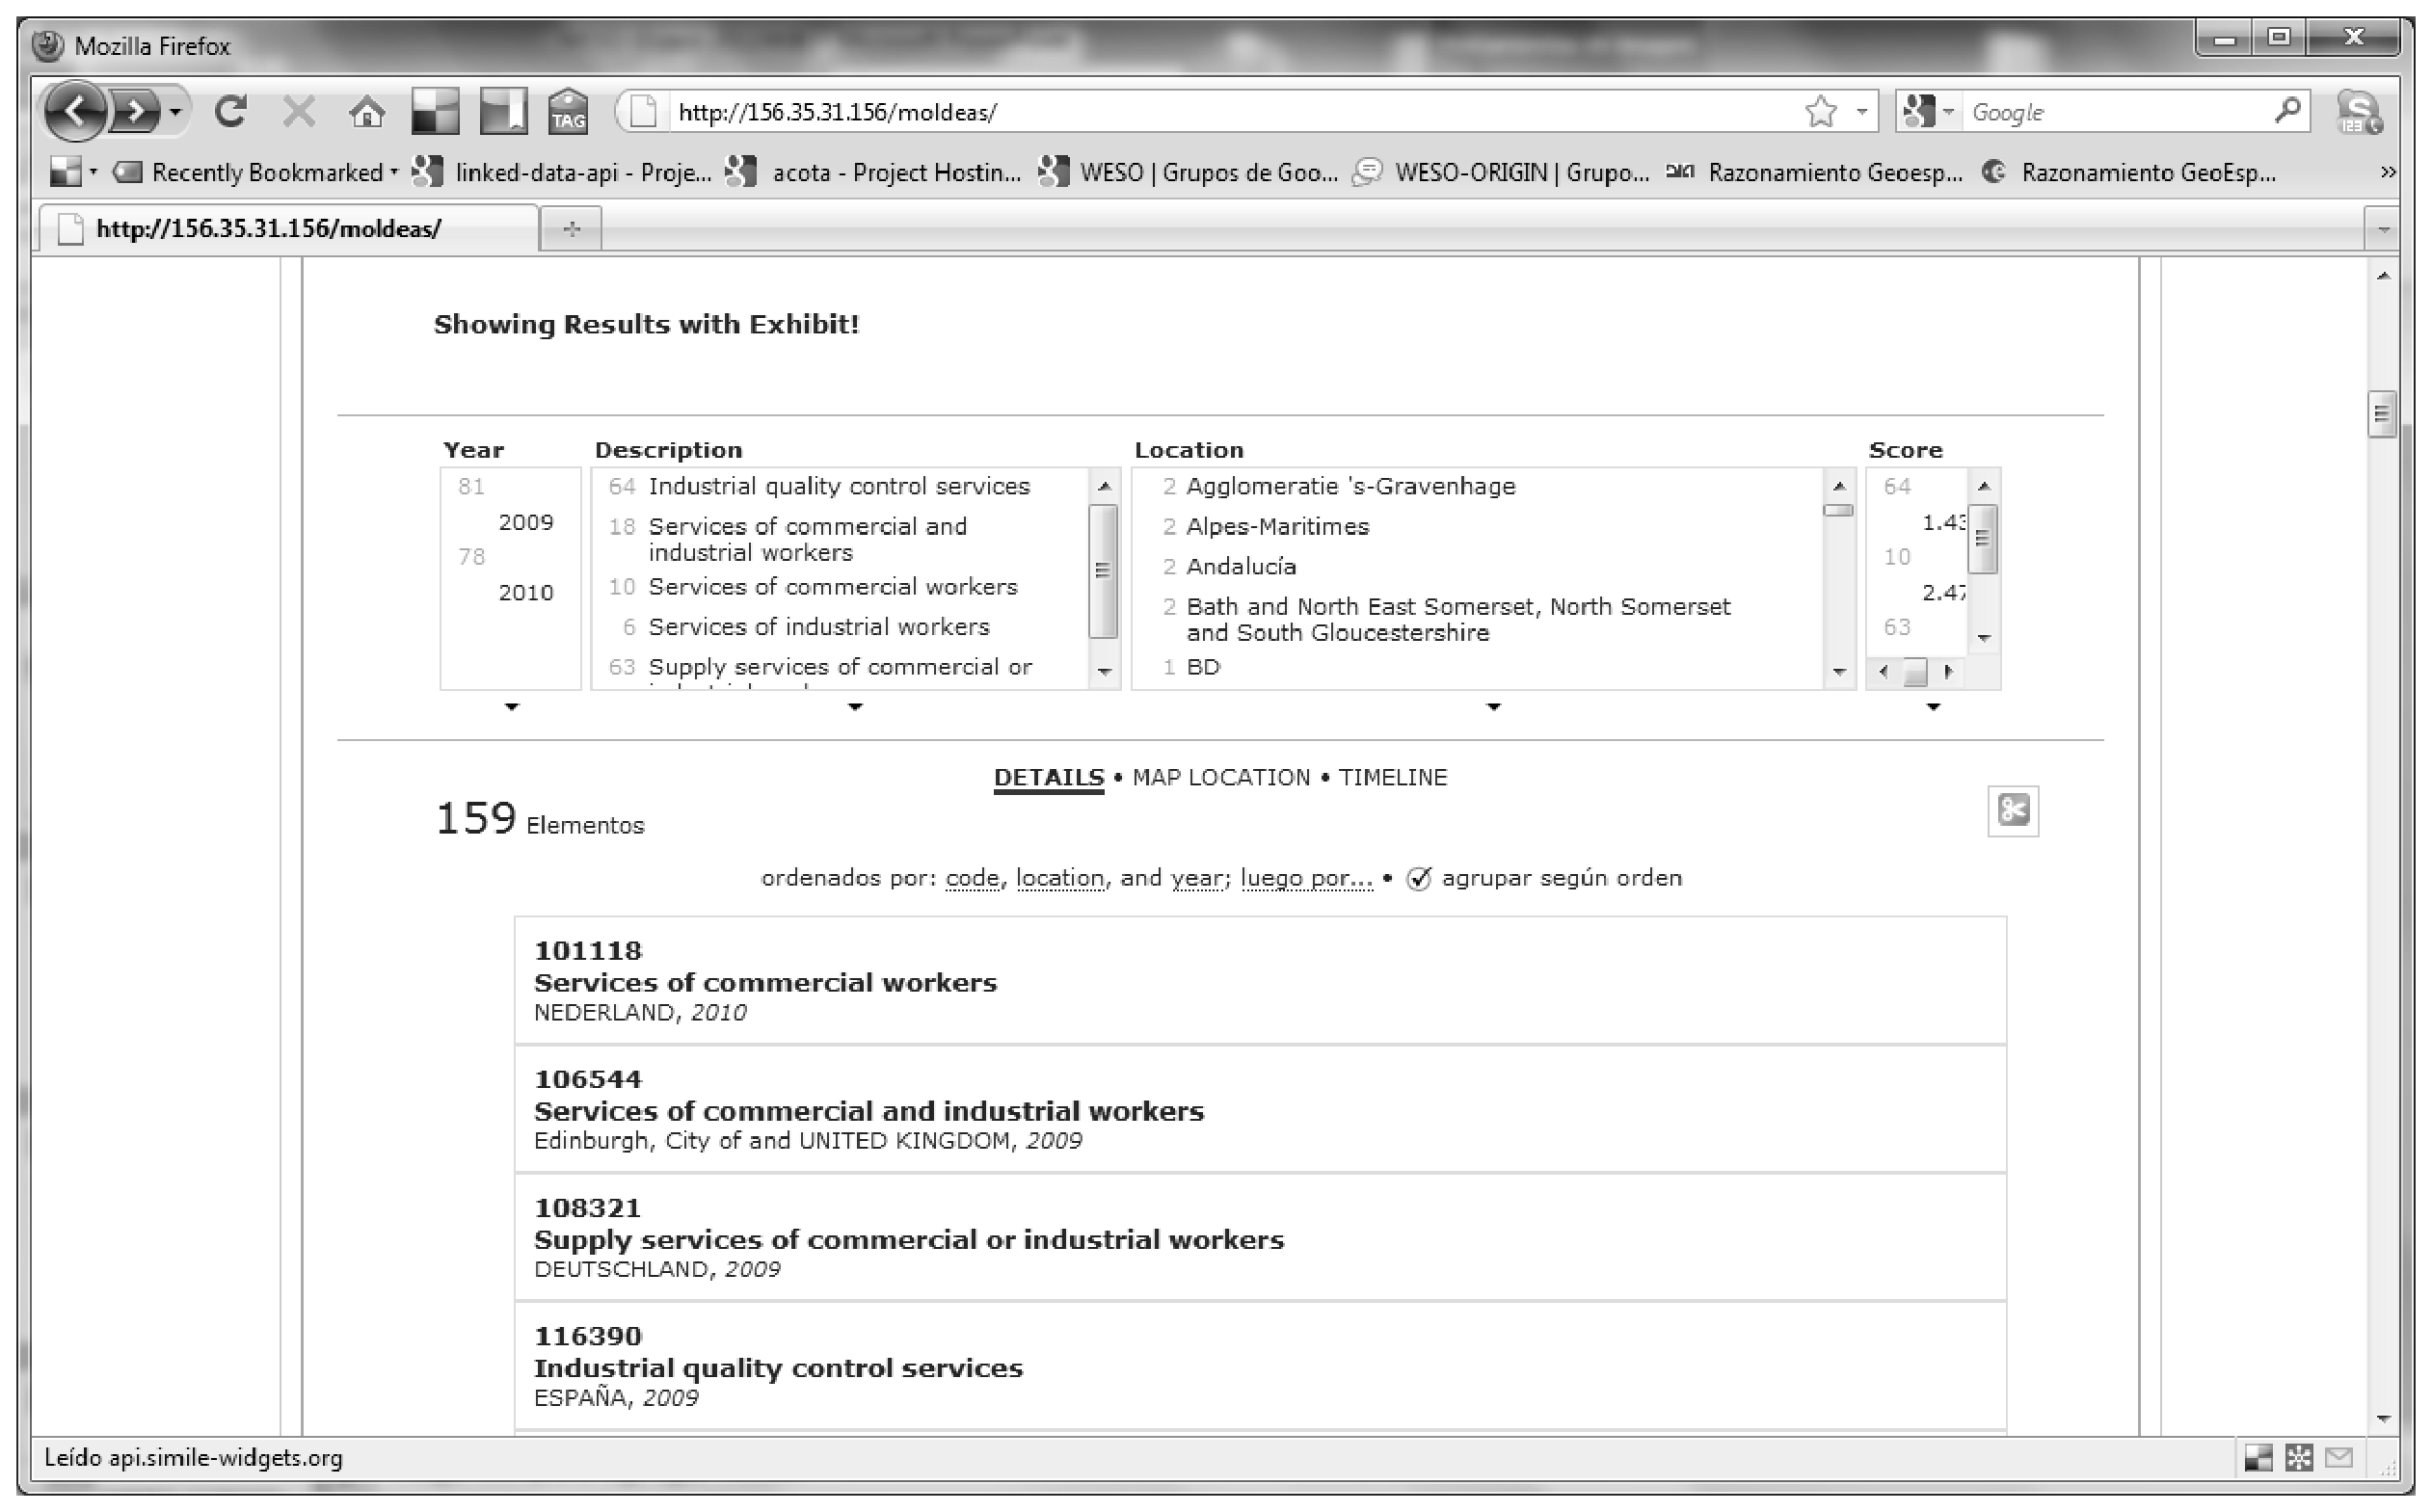
\includegraphics[width=10cm]{imgs/moldeas-results}

\end{figure}
}
\frame{
  \frametitle{MOLDEAS-Linked Data Frontend (Pubby)} 

\begin{figure}[!htb]
\centering
 	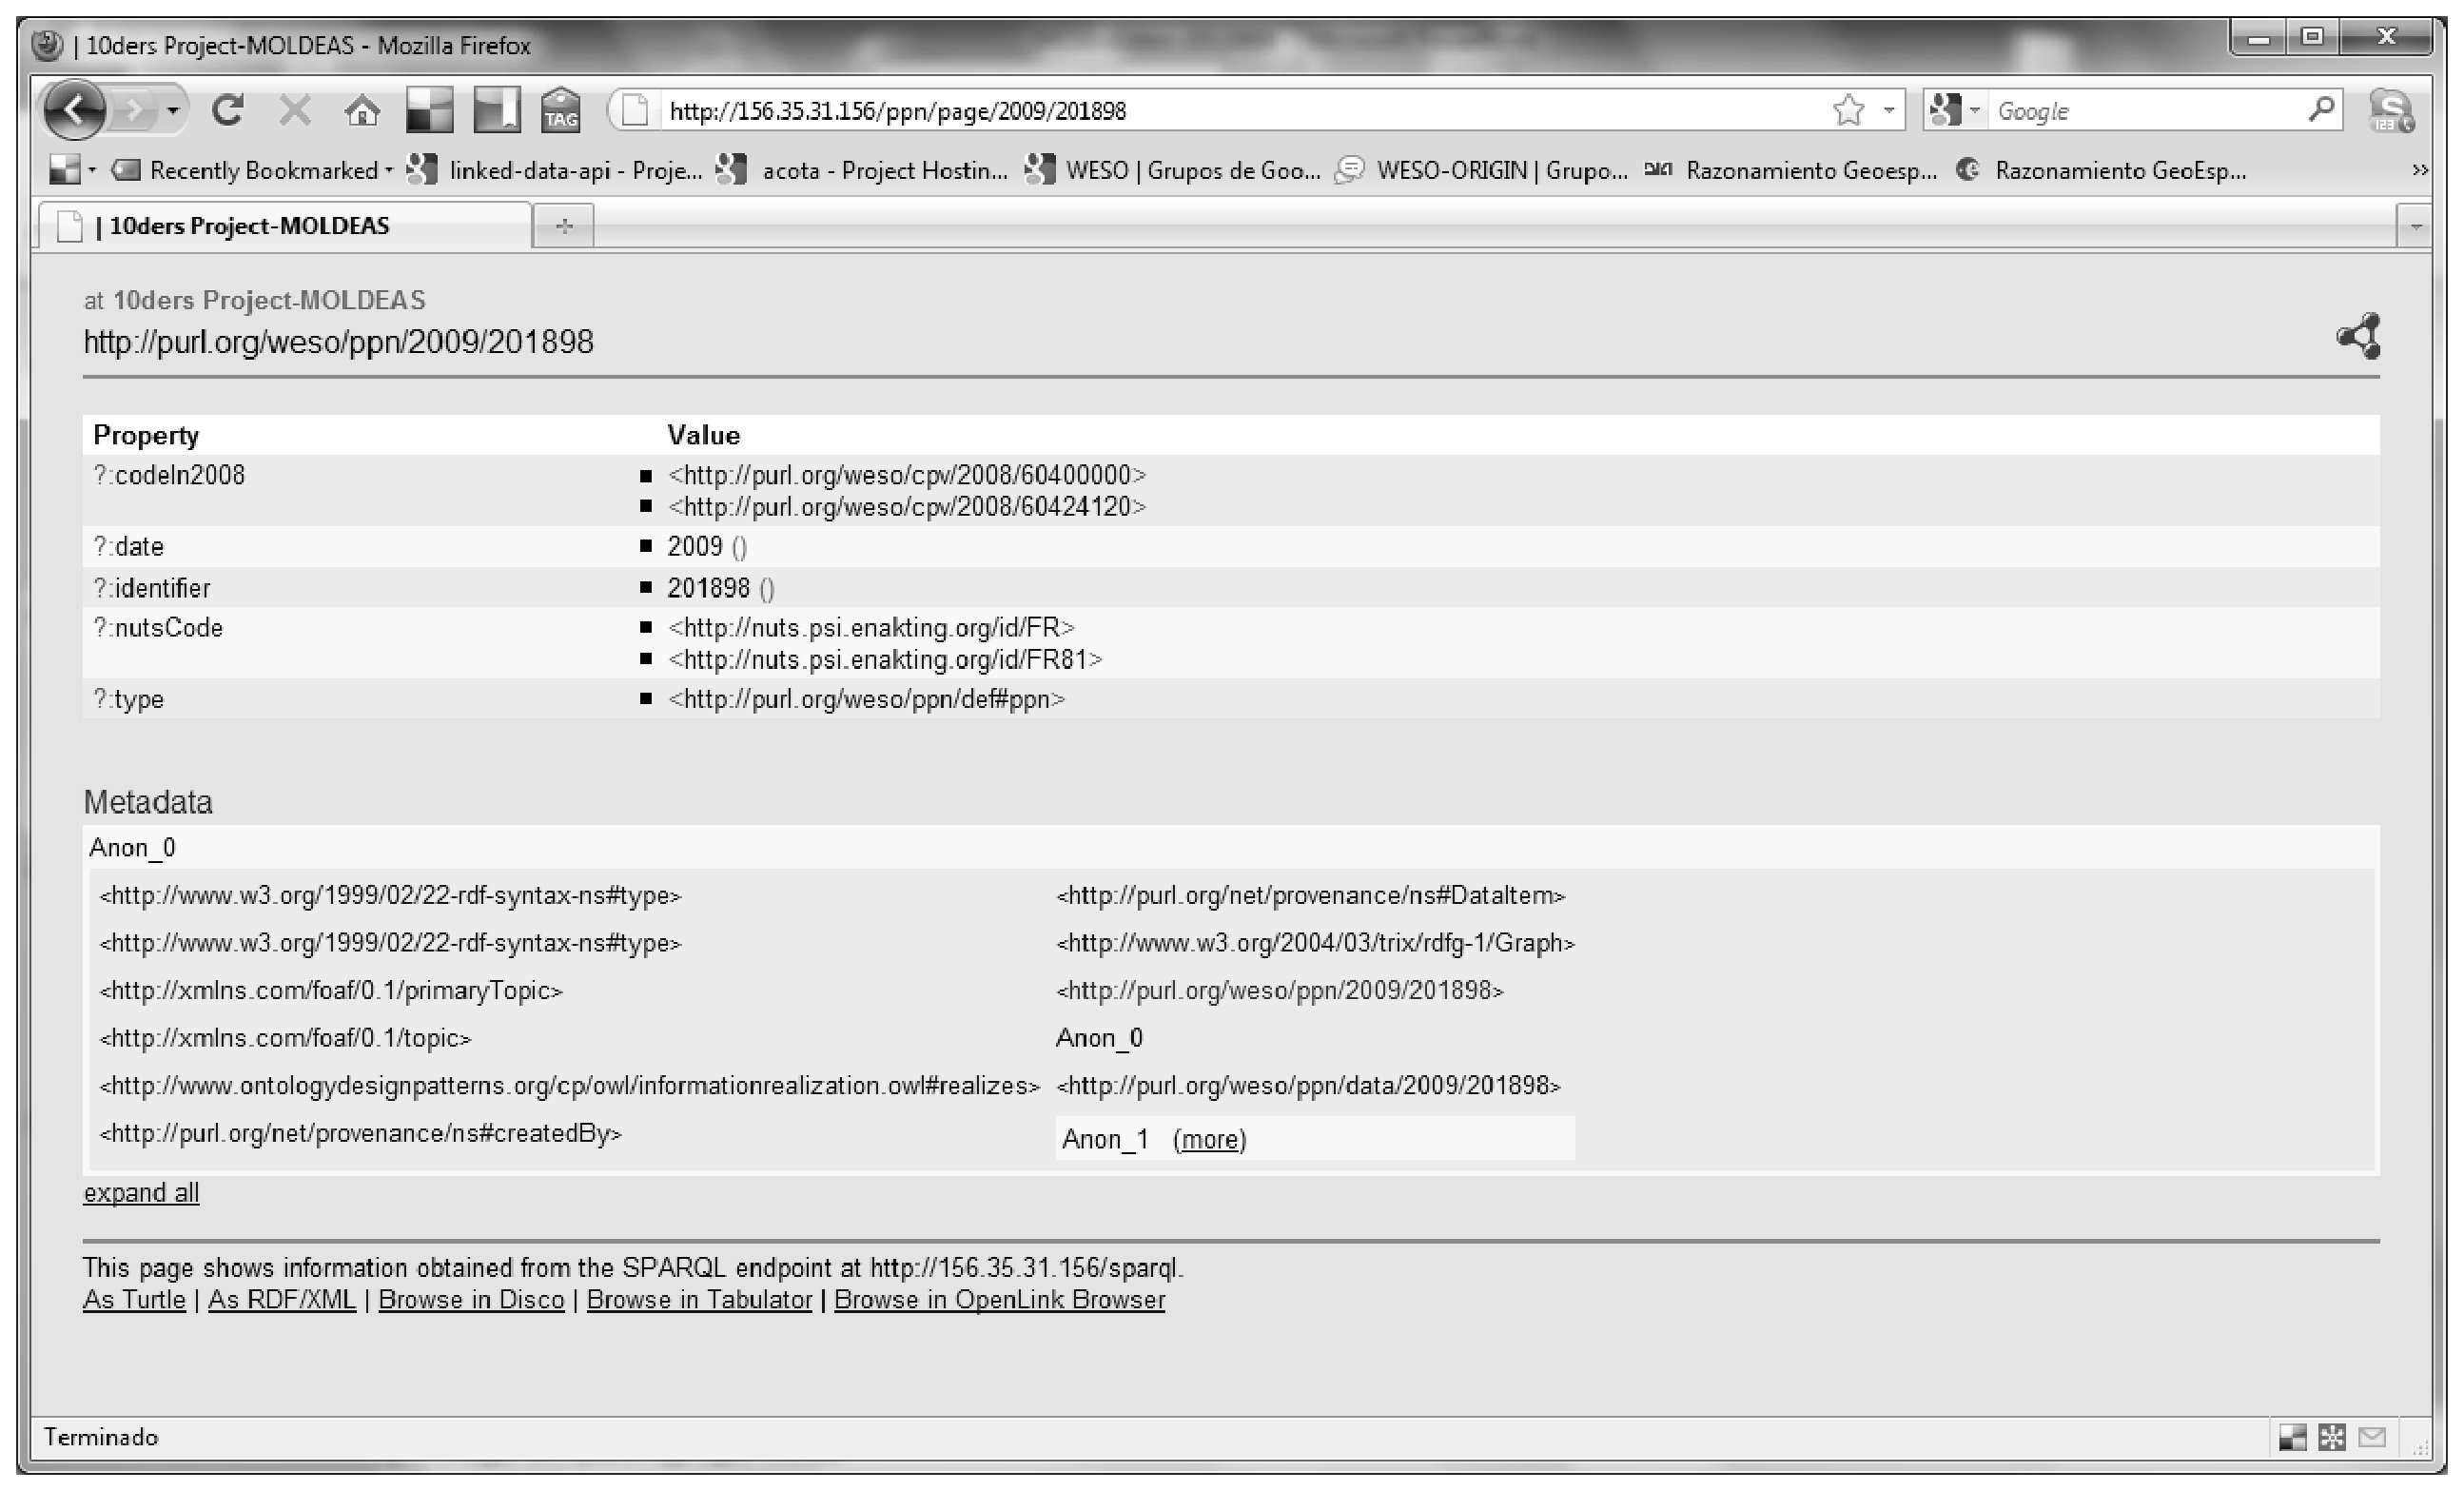
\includegraphics[width=10cm]{imgs/moldeas-pubby}

\end{figure}
}

% \frame{
%   \frametitle{MOLDEAS-Live queries (SNORQL)} 
% \begin{figure}[!htb]
% \centering
% 	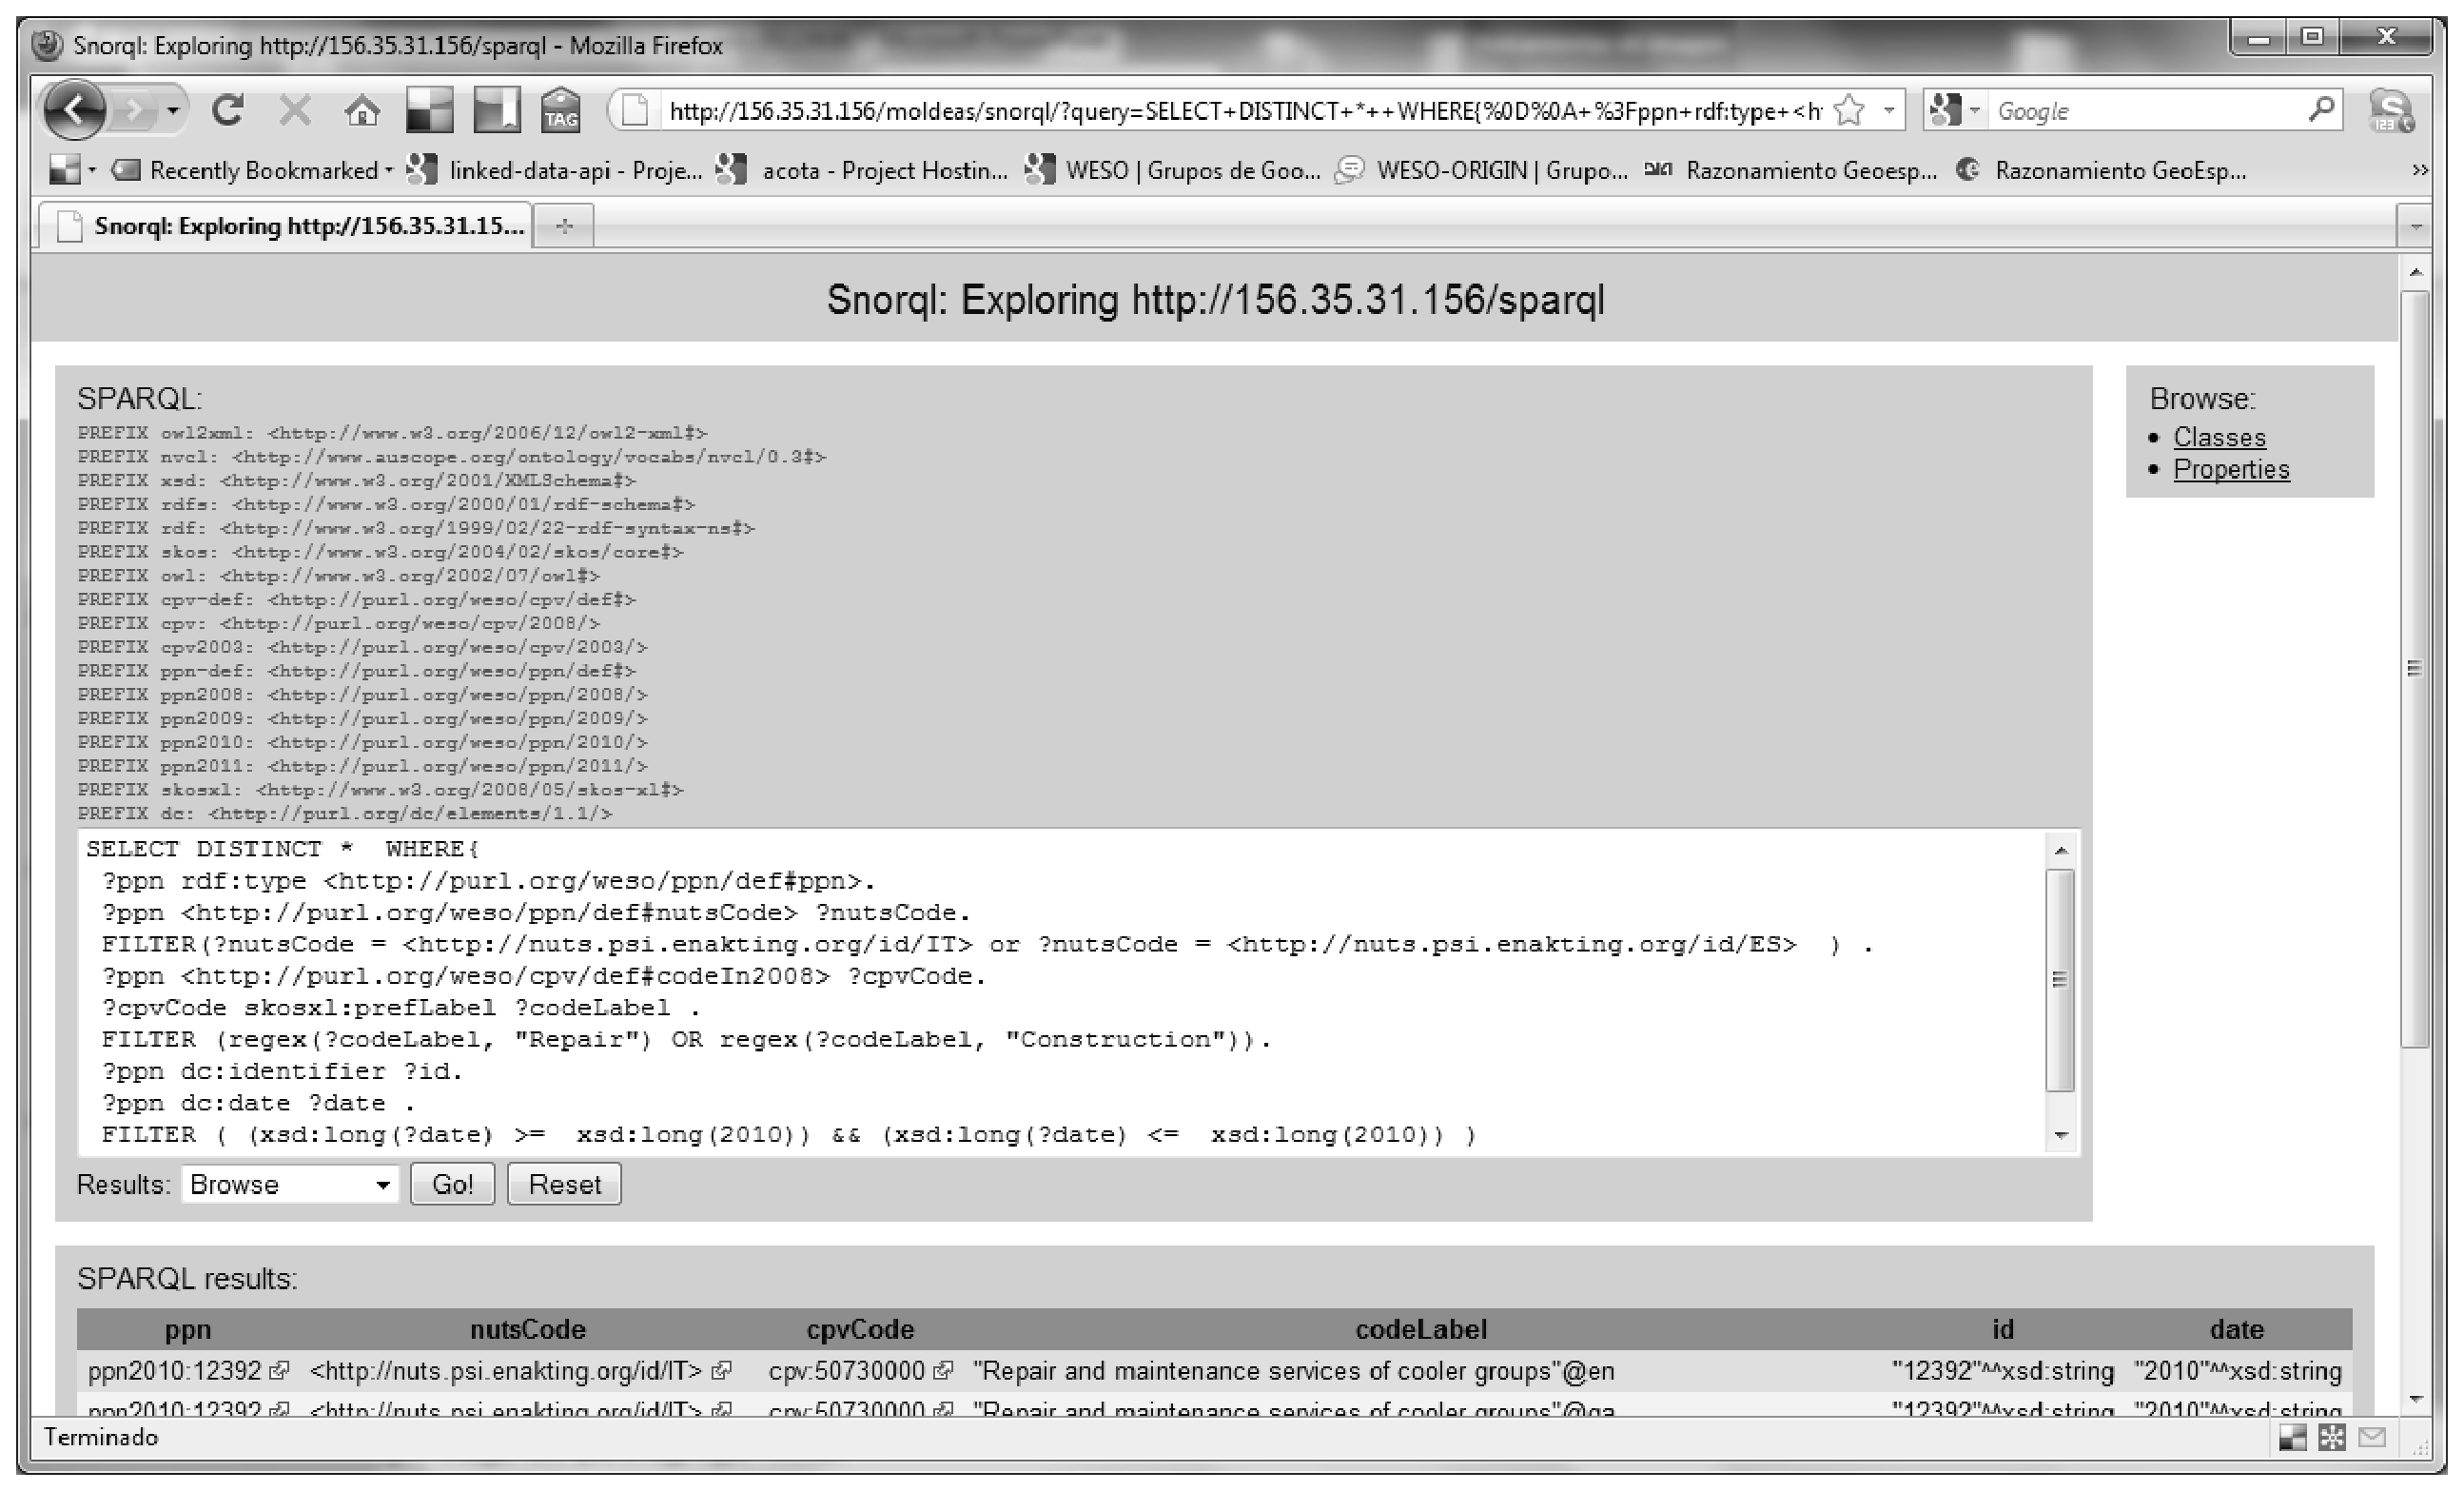
\includegraphics[width=10cm]{imgs/moldeas-snorql}
% \end{figure}
% 
% }

\section{Resultados y Evaluación}
\frame{
\large
\begin{enumerate}
\setcounter{enumi}{3}
 \item Resultados y Evaluación.
  \begin{itemize}
  \item Metodología.
  \item Expresividad y Cumplimiento de Criterios.
  \begin{enumerate}
   \item Punto de Vista Cuantitativo.
   \item Punto de Vista Cualitativo.
  \end{enumerate}
  \item Sistema MOLDEAS.
  \begin{enumerate}
   \item Consumo de Datos Enlazados Abiertos.
   \item Rendimiento de Consultas en SPARQL.
  \end{enumerate}
  \end{itemize}

\end{enumerate}

}


\frame{
  \frametitle{Metodología}

\begin{block}{Pasos de ejecución}
 \begin{enumerate}
\small
 \item Definición de los objetivos del experimento. 
\item Selección de una regla de asignación de las unidades experimentales a las condiciones de estudio. 
 \begin{itemize}
 \item Cualitativos: tipo de entorno hardware y software, etc.
   \item Cuantitativos: tamaño de la muestra, de la memoria y número de posibilidades de expresar una consulta.
\end{itemize}
 \item Especificación de las medidas de trabajo en cuanto a la respuesta.
 \item Especificación de un modelo.
 \item Ejecución de un experimento piloto. 
 \item Esquematización de los pasos a seguir. 
 \item Determinación del tamaño muestral.
 \item Revisión de las decisiones anteriores.
\end{enumerate}
\end{block}
}

\subsection*{Expresividad y Cumplimiento de Criterios}
\frame{
  \frametitle{Visión del experimento}

\begin{block}{Punto de Vista Cuantitativo}<1->
 ¿Cuál es la posibilidad de uso de datos enlazados para facilitar el \textbf{acceso} a un 
mayor número de recursos relacionados con los anuncios de licitación?
\end{block}

\begin{exampleblock}{Punto de Vista Cualitativo}<2->
Evaluación, grado de cumplimiento y comparación con otros enfoques de:
\begin{itemize}
 \item Principios de \opendata y \linkeddata.
 \item Buenas prácticas.
 \item Patrones de diseño.
 \item Características de pertenencia a la nube de datos enlazados y registro CKAN.
\end{itemize}
\end{exampleblock}
}

\frame{
\begin{block}{Expresividad}
Punto de Vista Cuantitativo.
\end{block}

}


\frame{
  \frametitle{Punto de Vista Cuantitativo}

\begin{block}{1-Definición de los objetivos del experimento}
\begin{enumerate}
 \item ¿Cuál es la expresividad actual, en términos de número de conceptos para realizar consultas, para el acceso a la información de anuncios de licitación?
 \item ¿Cuál es la ventaja de uso de un modelo RDF para la expresión y recuperación de la información de los anuncios de licitación?
 \item ¿Cómo favorecen los datos enlazados el aumento de expresividad en la ejecución de consultas y por tanto facilitan la recuperación de los 
anuncios de licitación? 
 \item ¿Cuál es el beneficio real del uso de datos enlazados para representar la información? 
 \item ¿Se incurre en algún error al aumentar la expresividad?
\end{enumerate}

\end{block}

}


\frame{
  \frametitle{Punto de Vista Cuantitativo}

\begin{block}{2-Selección de una regla de asignación de las unidades experimentales a las condiciones de estudio}<1->
\begin{enumerate}
\item Base documental $\mathcal{D}$ constituida por $1$ millón de anuncios de licitación.
\item Vocabulario controlado, $\mathcal{V}$, del CPV 2008, formado por $\#\mathcal{V} = 10357$ códigos/términos distintos.
\item Cada documento $d \in \mathcal{D}$, etiquetado con al menos un código $v \in \mathcal{V}$.
\item 9 Clasificaciones Estándar de Productos y Servicios.
\item Clasificación ``puente'': \textit{ProductOntology} (PO)
\end{enumerate}
\end{block}



}

\frame{
  \frametitle{Punto de Vista Cuantitativo}

\begin{block}{3-Especificación de las medidas de trabajo en cuanto a la respuesta}<1->
\begin{enumerate}
\item Nº de enlaces entre una PSC y el CPV 2008.
\item Nº de enlaces entre una PSC y el CPV 2008 a través de PO.
\item Ganancia de expresividad en términos porcentuales.
\end{enumerate}

\end{block}

\begin{exampleblock}{4-Especificación de un modelo}<2->
\begin{itemize}
\item El nuevo vocabulario controlado $\mathcal{V'}_{psc}$, enlazado con $\mathcal{V}_{psc}$, dispone de $\#\mathcal{V'}_{psc}$ términos.
\item La ganancia se calcula como: \begin{align}
\% =  \{ \langle (\#\mathcal{V'}_{psc}+\#\mathcal{V}) / \#\mathcal{V} \rangle - 1 \} * 100
\end{align}
\end{itemize}
\end{exampleblock}

}


\frame{
  \frametitle{Punto de Vista Cuantitativo}

\begin{block}{5-Ejecución de un experimento piloto}<1->
\begin{itemize}
 \item Sea $\mathcal{V} = \{ 1, 2, 3 \}$  y  $\mathcal{V}_{psc} = \{A, B, C, D, E\}$.
 \item El conjunto de pares enlaces es: $\{ (A,1), (B,2), (C,1) (E,2) \}$.
 \item Por tanto, el conjunto $\mathcal{V'}_{psc} = \{A, B, C, E\}$ y el \% de ganancia en expresividad será:
\begin{align}
\% =  \{ \langle (4+3) / 3 \rangle -1 \} * 100  =  133
\end{align}
\end{itemize}
\end{block}

\begin{exampleblock}{6-Esquematización de los pasos a seguir}<2->
\begin{enumerate}
\item Extracción de consultas en SPARQL para establecer el número de enlaces entre las mismas.
\item Procesamiento de los resultados mediante un \textit{script} para generar los resultados.
\end{enumerate}
\end{exampleblock}
}


\frame{
  \frametitle{Punto de Vista Cuantitativo}
\begin{alertblock}{Otros}
\begin{itemize}
 \item 7-Determinación del tamaño muestral (ya indicado en el punto 1).
 \item 8-Revisión de las decisiones anteriores.
\end{itemize}
\end{alertblock}
}



\frame{
    \frametitle{Punto de Vista Cuantitativo-Resultados Parciales}
\small
\begin{longtable}[c]{|l|l|l|l|l|p{1cm}|p{1cm}|} 
\hline
  $\mathcal{V}_{psc}$ & $\#\mathcal{V}_{psc}$  & $\#\mathcal{V'}_{psc}$ &$\#\mathcal{V'''}_{psc}$ &  $\%$ real &  $\%$ real \textit{PO}  &  $\%$ máx.   \\\hline
\endhead
CPV 2003 	& $8323$  	& $462$		& $8312$ 	& $4.46$ 	& $80.25$	& $80.36$  \\ \hline
CN 2012  	& $14552$	& $2390$	& $2390$ 	& $23.07$	& $23.07$	& $140.50$  \\ \hline
CPC 2008 	& $4408$	& $4402$   	& $4403$	& $42.50$	& $42.51$ 	& $42.56$  \\ \hline
CPA 2008 	& $5429$	& $5399$   	& $5410$	& $52.12$	& $52.23$	& $52.41$  \\ \hline
ISIC v4  	& $766$		& $765$   	& $765$ 	& $7.38$ 	& $7.38$	& $7.39$    \\ \hline
NAICS 2007 	& $2328$	& $2300$ 	& $2300$	& $22.20$	& $22.20$	& $22.47$  \\ \hline
NAICS 2012 	& $2212$	& $2186$ 	& $2186$	& $21.10$	& $21.10$	& $21.35$  \\ \hline
SITC v4 	& $4017$	& $3811$   	& $3820$	& $36.79$	& $36.88$	& $38.78$  \\ \hline
\multicolumn{7}{|c|}{\textbf{...}} \\ \hline
\hline
\end{longtable}
}

\frame{
  \frametitle{Punto de Vista Cuantitativo-Resultados Totales}
\small
\begin{longtable}[c]{|l|l|l|l|l|l|p{1cm}|} 
\hline
  \multicolumn{7}{|c|}{\textbf{Total}} \\ \hline
  $\mathcal{V}_{psc}$ & $\#\mathcal{V}_{psc}$  & $\#\mathcal{V'}_{psc}$ &$\#\mathcal{V'''}_{psc}$ &  $\%$ real &  $\%$ real \textit{PO}  &  $\%$ máx.   \\\hline
\endhead
$\star$ & $42035$ 		& $21715$   	& $29586$	& $209.66$ 	& $285.66$	& $405.86$ \\ \hline
\multicolumn{7}{|c|}{\textbf{Añadiendo enlaces entre CPV 2008 y \textit{Product Ontology-PO}}} \\ \hline
\textit{PO}& $\infty$	& $10000$   	& N/A	& $96.55$	& $96.55$ 	& $\infty$  \\ \hline
\multicolumn{7}{|c|}{\textbf{Total con vocabulario de \textit{Product Ontology}}} \\ \hline
$\star$	 & $\infty$	& $31715$   	& 39586	& $306.21$	& $382.21$	& $\infty$ \\ \hline
\hline
\end{longtable}

}


\frame{
  \frametitle{Punto de Vista Cuantitativo-Resultados}

\begin{figure}[!htb]
\centering
	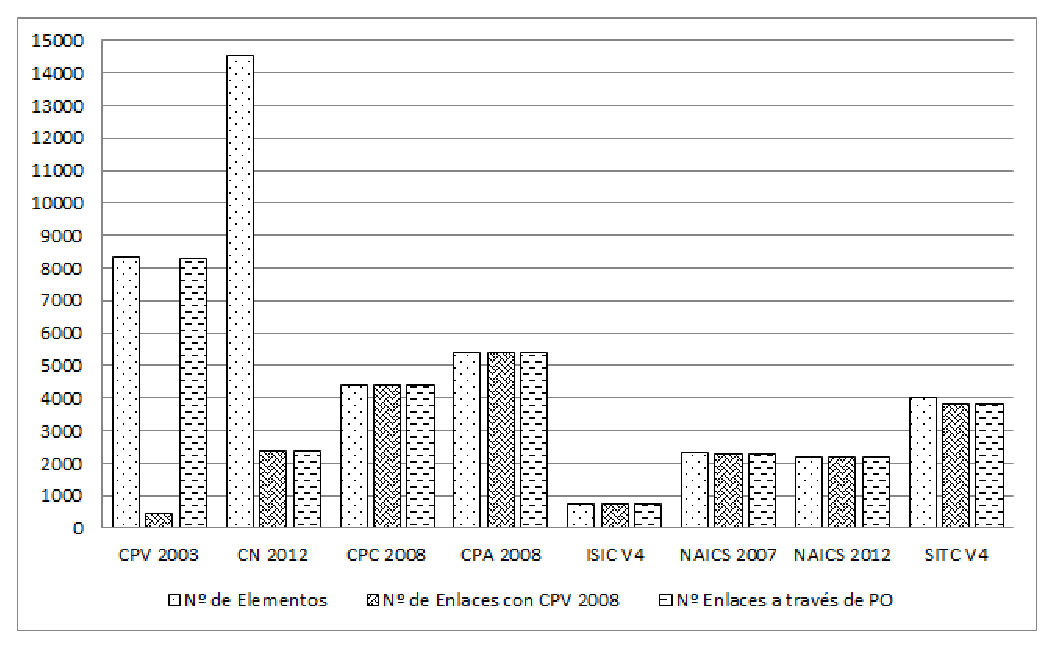
\includegraphics[width=10cm]{./imgs/pscs-enlaces}
\caption{Número de Elementos y Enlaces entre las PSCs y el CPV 2008.}
\end{figure}

}

\frame{
  \frametitle{Punto de Vista Cuantitativo-Resultados}

\begin{figure}[!htb]
\centering
	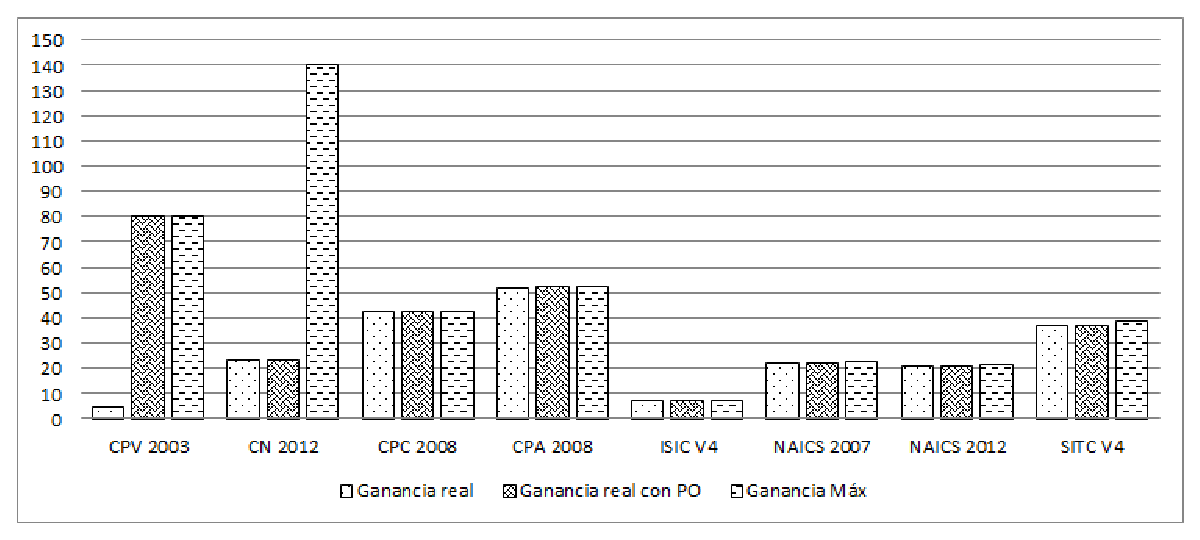
\includegraphics[width=10cm]{./imgs/pscs-ganancia}
\caption{Ganancia en expresividad.}
\end{figure}

}

\frame{
  \frametitle{Punto de Vista Cuantitativo-Resultados}

\begin{block}{Valoración}
 \begin{enumerate}
  \item Extensión del CPV 2008, $10357$ términos, hasta:
 \begin{itemize}
  \item $21715$ términos, con enlaces entre las PSCs y el CPV 2008.
  \item $29586$ términos, con enlaces entre las PSCs y el CPV 2008 a través de \textit{PO}.
 \end{itemize}
  \item Se establece un:
   \begin{itemize}
    \item \textbf{$8.65\%$} y \textbf{$6.64\%$} (PO) de enlaces exactos.
    \item \textbf{$91.35\%$} y \textbf{$93.36\%$} (PO) de enlaces automáticos.
   \end{itemize}
 \item Cifras de ganancia:
  \begin{itemize}
  \item Real: $209.66\%$.
  \item Real con \textit{PO}: $285.66\%$
  \item Máximo: $405.86\%$.
 \end{itemize}
  \item Los enlaces y la reconciliación de entidades se realizan bajo un umbral $\mu$ ($n$ primeros resultados normalizados).
 \end{enumerate}
\end{block}


}

\frame{
  \frametitle{Punto de Vista Cuantitativo-Resultados}

\begin{figure}[!htb]
\centering
	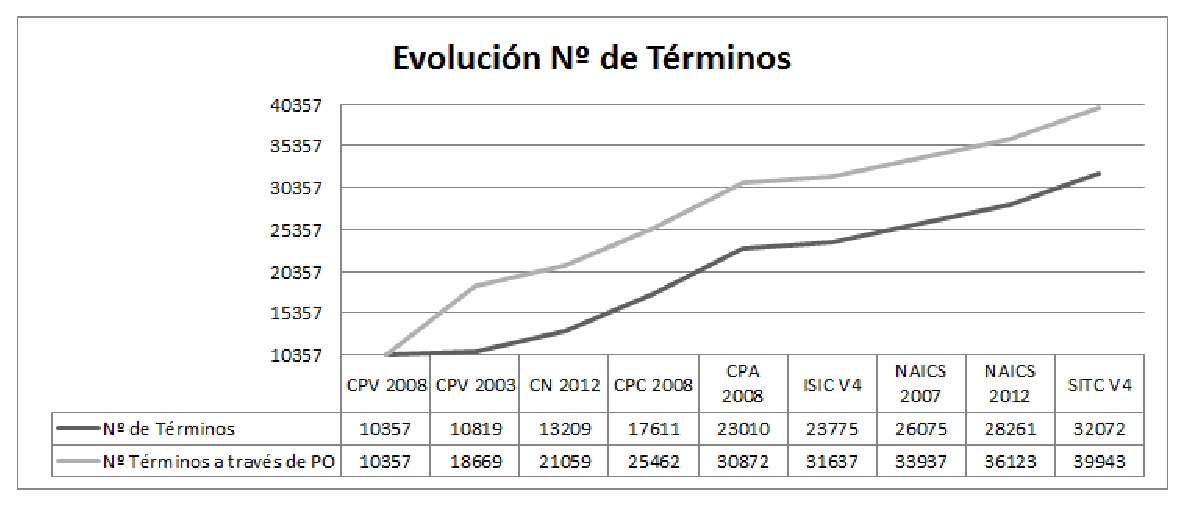
\includegraphics[width=11cm]{./imgs/evo-n-terminos}
\caption{Evolución Número de Términos.}
\label{fig:eval-n-terminos}
\end{figure}

}


\frame{
  \frametitle{Punto de Vista Cuantitativo-Conclusiones}

\begin{exampleblock}{Puntos Clave}
\begin{itemize}
 \item \textbf{Aumento} del \textbf{vocabulario de entrada} del CPV 2008 con \linkeddata.
 \item \textbf{Mejora} de la \textbf{expresividad} para la realización de consultas en SPARQL.
 \item \textbf{Incremento} del número de \textbf{anuncios} de licitación a los que se puede \textbf{acceder}.
 \item \textbf{Establecimiento} de una \textbf{fórmula} para el cálculo de la \textbf{ganancia} del enlazado de datos.
\end{itemize}
\end{exampleblock}
}

%%%%%%%%%
%%%%%%%%	punto de vista cualitativo
%%%%%%%%


\frame{
\begin{exampleblock}{Cumplimiento de Criterios}
Punto de Vista Cualitativo. 
\end{exampleblock}
}



\frame{
  \frametitle{Punto de Vista Cualitativo}

\begin{block}{1-Definición de los objetivos del experimento}
\begin{enumerate}
 \item ¿El ciclo de vida seguido y los datos generados certifican la aplicación de buenas prácticas y principios de \linkeddata?
 \item ¿Qué nivel del modelo de 5 $\star$ se puede establecer?
 \item ¿Qué porcentaje de patrones de diseño se han aplicado en los datos generados?
 \item ¿Los datos generados pueden pertenecer a la nube de datos enlazados abiertos?
 \item ¿Los datos generados pueden pertenecer a un registro CKAN? 
 \item ¿Se certifica el cumplimiento de los principios de \opendata?
 \item ¿Se puede asegurar que los datos son enlazados y abiertos?
 \item ¿Qué beneficios se obtienen del cumplimiento de estos objetivos?
\end{enumerate}

\end{block}

}

\frame{
  \frametitle{Punto de Vista Cualitativo}

\begin{block}{2-Selección de una regla de asignación de las unidades experimentales a las condiciones de estudio}<1->
\begin{enumerate}
\item \textit{Dataset} RDF de los anuncios de licitación pública.
\begin{itemize}
 \item Boletines y Publicaciones oficiales: TED y BOE.
 \item Plataformas de contratación: AGE.
 \item Servicios de terceros: Euroalert.net y Licitaciones.es
 \item Basados en semántica: LOTED.
\end{itemize}
\item \textit{Dataset} RDF de las PSCs.
\begin{itemize}
 \item Publicaciones oficiales: UE, ONU, etc.
 \item Servicios de terceros.
\end{itemize}
\item \textit{Dataset} RDF de las organizaciones.
\begin{itemize}
 \item Boletines y Publicaciones oficiales: TED y BORME.
 \item Plataformas de contratación: AGE.
 \item Servicios y BBDD de terceros.
 \item Basadas en \opendata: OpenCorporates.
\end{itemize}
\end{enumerate}
\end{block}


}


\frame{
  \frametitle{Punto de Vista Cualitativo}

\begin{block}{3-Especificación de las medidas de trabajo en cuanto a la respuesta}
\begin{enumerate}
 \item Valor positivo, \si, si es un criterio que debe tener y se cumple (\textbf{173}).
 \item Valor negativo, \no, si es un criterio que debe tener y no se cumple (\textbf{0}).
 \item Valor no aplicable, \na, si es un criterio que se desconoce, que se solapa con otro o no está asociado a ese enfoque (\textbf{23}).
\end{enumerate}
\end{block}

}


\frame{
  \frametitle{Punto de Vista Cualitativo}
\begin{exampleblock}{Diseño de Tablas de Validación}
\begin{itemize}
\item $T^{1}$-Tabla de Validación de Características \linkeddata.
\item $T^{2}$-\ldots de \textit{Linked Data Patterns}.
\item $T^{3}$-\ldots de Principios de \linkeddata.
\item $T^{3}_1$-\ldots del Modelo $\star$.
\item $T^{4}$-\ldots de Principios de \opendata.
\item $T^{4}_1$-\ldots sobre Características de \opendata.
\item $T^{5}$-\ldots sobre Características para pertenecer a la nube de \lod.
\item $T^{6}$-\ldots para registrar el \dataset en CKAN.
\end{itemize}
\end{exampleblock}

}

\frame{
  \frametitle{Punto de Vista Cualitativo}

\begin{block}{4-Especificación de un modelo}<1->
No aplicable.
\end{block}

\begin{exampleblock}{5-Ejecución de un experimento piloto}<2->
Valoración inicial con sólo un conjunto de datos.
\end{exampleblock}

\begin{alertblock}{6-Esquematización de los pasos a seguir}<3->
\begin{enumerate}
 \item Establecimiento del modelo de referencia, con los valores admitidos.
 \item Revisión uno a uno de los criterios.
 \item Agregación de los resultados y valoraciones.
 \item Extracción de estadísticas, contraste de hipótesis, validación y evaluación.
\end{enumerate}
\end{alertblock}
}


\frame{
  \frametitle{Punto de Vista Cualitativo}
\begin{block}{Otros}
\begin{itemize}
 \item 7-Determinación del tamaño muestral (ya indicado en el punto 1).
 \item 8-Revisión de las decisiones anteriores.
\end{itemize}
\end{block}
}





\frame{
  \frametitle{Punto de Vista Cualitativo-Resultados en \%}
\small
\begin{longtable}[c]{|p{2.25cm}|c|c|c|c|c|c|c|c|}
\hline
\textbf{Versión}&$T^{1}$ & $T^{2}$& $T^{3}$ & $T^{3}_1$ & $T^{4}$ & $T^{4}_1$ &$T^{5}$ & $T^{6}$ \\ \hline
\endhead
 \multicolumn{9}{|c|}{\textbf{Anuncios de Licitación}} \\ \hline
 \textbf{TED}	     			& $65$ & \na & $100$ & $100$ & $75$ & $78,57$ & \na & \na \\ \hline
 \textbf{Plataforma de Contratación}	& $75$ & \na & $100$ & $100$ & $87,5$ & $78,57$ & \na & \na \\ \hline 
 \textbf{BOE}	     			& $52,63$ & \na & $100$ & $100$ & $100$ & $76,92$ & \na & \na\\ \hline 
 \textbf{Servicios Externos}	     	& $60$ & \na & $100$ & $100$ & $62,5$ & $66,66$ & \na & \na \\ \hline 
 \textbf{LOTED}	     			& $59,32$ & $74,19$ & $100$ & $100$ & $100$ & $85,71$ & $100$ & \na \\ \hline 
 \textbf{MOLDEAS}	     		& $88,52$ & $91,18$ & $100$ & $100$ & $100$ & $100$ & $100$ & \na \\ \hline 
\hline
\end{longtable} 

}

\frame{
  \frametitle{Punto de Vista Cualitativo-Resultados en \%}
\small
 \begin{longtable}[c]{|p{2cm}|c|c|c|c|c|c|c|c|}
\hline
\textbf{Versión}&$T^{1}$ & $T^{2}$& $T^{3}$ & $T^{3}_1$ & $T^{4}$ & $T^{4}_1$ &$T^{5}$ & $T^{6}$ \\ \hline
\endhead
 \multicolumn{9}{|c|}{\textbf{Catálogo de Clasificaciones de Productos}} \\ \hline
 \textbf{CSV/ MSExcel} 			&$69,23$ & \na & \na & $100$ & $100$ & $42,86$ & \na & \na \\ \hline 
 \textbf{Servicios on-line}  		&$50$ & \na & \na & \na & $71,43$ & $38,46$ & \na & \na \\ \hline 
 \textbf{MOLDEAS}			&$88,52$ & $100$ & $100$ & $100$ & $100$ & $100$ & $100$ & $100$ \\ \hline 
\hline
\end{longtable} 


}
\frame{
  \frametitle{Punto de Vista Cualitativo-Resultados en \%}
\small
\begin{longtable}[l]{|p{2.25cm}|c|c|c|c|c|c|c|c|}
\hline
\textbf{Versión}&$T^{1}$ & $T^{2}$& $T^{3}$ & $T^{3}_1$ & $T^{4}$ & $T^{4}_1$ &$T^{5}$ & $T^{6}$ \\ \hline
\endhead
 \multicolumn{9}{|c|}{\textbf{Organizaciones}} \\ \hline
 \textbf{TED} 				& $50$ & \na & \na & $100$ & $75$ & $71,43$ & \na & \na \\ \hline 
 \textbf{Plataforma de Contratación} 	& $76,47$ & \na & $100$ & $20$ & $100$ & $85,71$ & \na & \na\\ \hline 
 \textbf{BORME}			 	& $100$ & \na & \na & $100$ & $100$ & $92,85$ & \na & \na \\ \hline 
 \textbf{Servicios Externos} 		& $60$ & \na & $100$ & $100$ & $12,5$ & $50$ & \na & \na \\ \hline 
 \textbf{BBDD externa} 			& $100$ & \na & \na & \na & $16,67$ & $71,43$ & \na & \na \\ \hline 
 \textbf{Open Corporates} 	 	& $61,40$ & $67,74$ & $100$ & $100$ & $100$ & $92,86$ & $100$ & \na\\ \hline 
 \textbf{MOLDEAS} 		 	& $88,52$ & $91,18$ & $100$ & $100$ & $100$ & $100$ & $100$ & \na \\ \hline 
\hline
\end{longtable} 

}

\frame{
  \frametitle{Punto de Vista Cualitativo-Resultados}

\begin{figure}[!htb]
\centering
	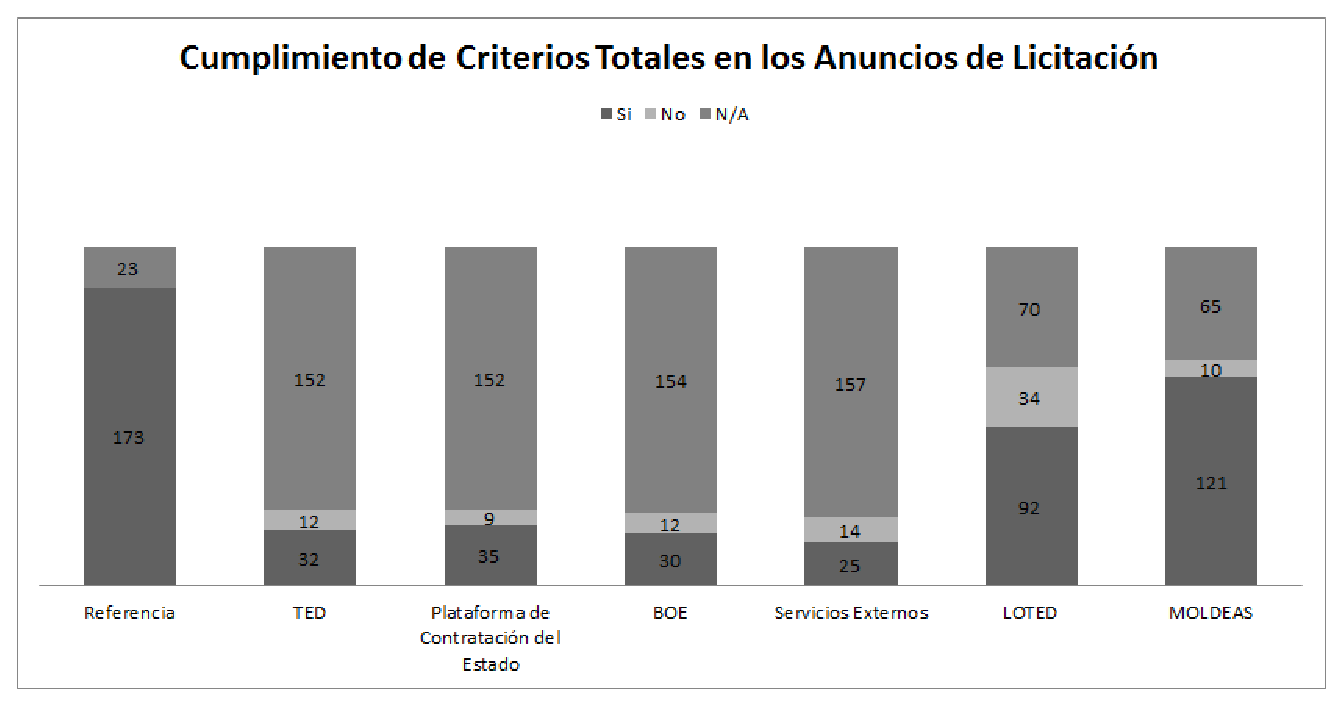
\includegraphics[width=11cm]{./imgs/criterios-total-ppn}
\end{figure}

}

\frame{
  \frametitle{Punto de Vista Cualitativo-Resultados}

\begin{figure}[!htb]
\centering
	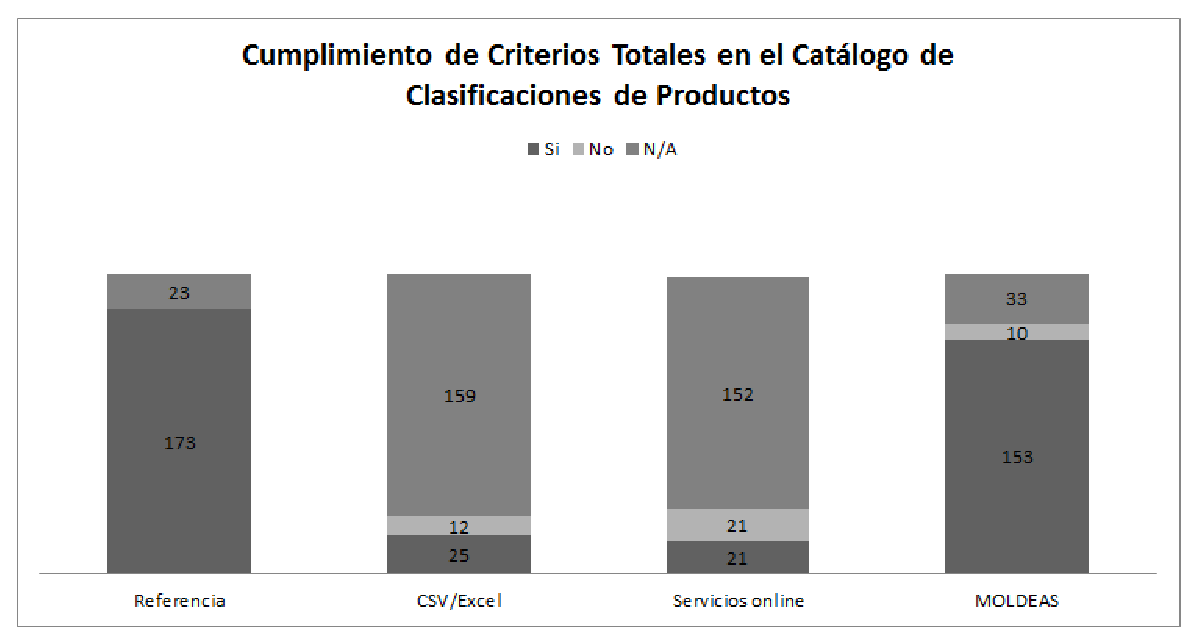
\includegraphics[width=11cm]{./imgs/criterios-total-pscs}
\end{figure}

}
\frame{
  \frametitle{Punto de Vista Cualitativo-Resultados}
\begin{figure}[!htb]
\centering
	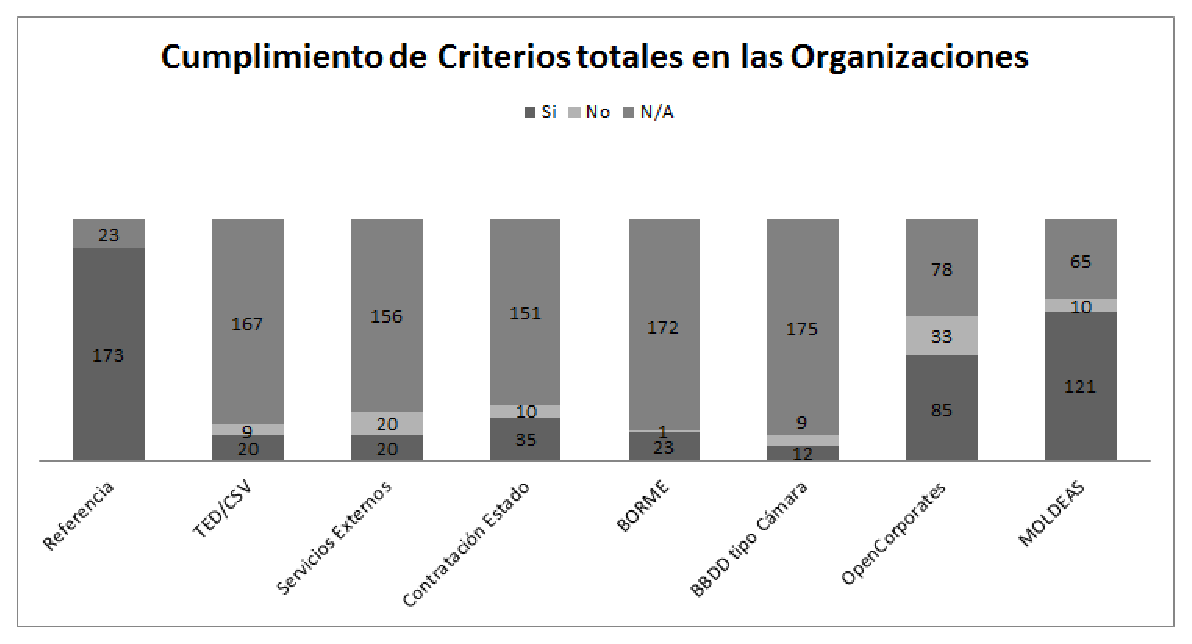
\includegraphics[width=11cm]{./imgs/criterios-total-orgs}
\end{figure}

}



\frame{
  \frametitle{Punto de Vista Cualitativo-\linebreak Resultados en \% \si entre aplicables}
\small
\begin{longtable}[c]{|p{2.25cm}|c|c|c||c||c|} 
\hline
 \textbf{Versión} & \si&\no&\na & \textbf{Total} & \textbf{\% \si entre aplicables} \\\hline
\endhead
    \textbf{Referencia} & 173 & 0 & 23 & 196& 100 \\ \hline \hline
 \multicolumn{6}{|c|}{\textbf{Anuncios de Licitación}} \\ \hline   
     \textbf{TED} & 32 & 12 & 152 &`` & $72.72$\\ \hline 
     \textbf{Plataforma de Contratación} & 35 & 9 & 152 &`` & $79.54$\\ \hline 
    \textbf{BOE} & 30 & 12 & 154 &`` & $71.42$\\ \hline 
    \textbf{Servicios Externos} & 25 & 14 & 157 &`` & $64.10$\\ \hline 
    \textbf{LOTED} & 92 & 34 & 70 &`` & $73.01$\\ \hline 
     \textbf{MOLDEAS} & 121 & 10 & 65 &`` & $92.36$\\ \hline 
\hline
\end{longtable}
}


\frame{
  \frametitle{Punto de Vista Cualitativo-\linebreak Resultados en \% \si entre aplicables}
\small
\begin{longtable}[c]{|p{2cm}|c|c|c||c||c|} 
\hline
 \textbf{Versión} & \si&\no&\na & \textbf{Total} & \textbf{\% \si entre aplicables} \\\hline
\endhead
    \textbf{Referencia} & 173 & 0 & 23 & 196& 100 \\ \hline \hline
 \multicolumn{6}{|c|}{\textbf{Catálogo de Clasificaciones de Productos}} \\ \hline
    \textbf{CSV/ MSExcel} &  25 & 12 & 159 &`` & $67.56$\\ \hline 
     \textbf{Servicios on-line} &  21 & 21 & 154 &`` & $50$\\ \hline 
    \textbf{MOLDEAS} &  166 & 7 & 23 &`` & $93.86$\\ \hline 

\hline
\end{longtable}
}


\frame{
  \frametitle{Punto de Vista Cualitativo-\linebreak Resultados en \% \si entre aplicables}
\small
\begin{longtable}[c]{|p{2.25cm}|c|c|c||c||c|} 
\hline
 \textbf{Versión} & \si&\no&\na & \textbf{Total} & \textbf{\% \si entre aplicables} \\\hline
\endhead
    \textbf{Referencia} & 173 & 0 & 23 & 196& 100 \\ \hline \hline
 \multicolumn{6}{|c|}{\textbf{Organizaciones}} \\ \hline
    \textbf{TED} & 20 & 9 & 167 &`` & $68.96$\\ \hline 
    \textbf{Plataforma de Contratación}  & 35 & 10 & 151 &`` & $77.77$ \\ \hline 
    \textbf{BORME}  & 23 & 1 & 172 &``& $95.83$\\ \hline 
    \textbf{Servicios Externos}  & 20 & 20 & 156 &`` & $50$\\ \hline   
    \textbf{BBDD externa}  & 12 & 9 & 175 &`` & $57.14$\\ \hline 
    \textbf{Open Corporates}  & 85 & 33 & 78  &`` & $72.03$\\ \hline 
    \textbf{MOLDEAS}  & 121 & 10 & 65 &`` & $92.36$\\ \hline 
\hline
\end{longtable}
}









\frame{
  \frametitle{Punto de Vista Cualitativo-Resultados}

\begin{block}{Valoración}
 \begin{enumerate}
\item El ciclo de vida asegura los principios y criterios de \linkeddata y \opendata.
\item Se establece un nivel de $5\star$ para los \datasets transformados.
\item Se ha aplicado un alto porcentaje de patrones de diseño, calidad implícita para la reutilización de datos.
\item Los \datasets transformados pueden pertenecer a la nube de \lod y a un registro CKAN.
\item En general, el enfoque de MOLDEAS mejora cualitativamente la información y datos respecto a otros enfoques.
 \end{enumerate}
\end{block}
}


\frame{
  \frametitle{Punto de Vista Cualitativo-Conclusiones}
\begin{exampleblock}{Puntos Clave}
\begin{itemize}
\small
 \item \textbf{Mejora} \textbf{cualitativa} la información y datos.
 \item \textbf{Aumento} de la visión global de los datos, \textbf{expresividad} y \textbf{estructuración}.
 \item \textbf{Aplicación} intensiva de \textbf{estándares}.
 \item \textbf{Incremento} del \textbf{conocimiento} en el dominio de \eproc.
 \item \textbf{Impulso} de la \textbf{reutilización} de la \textbf{información} y datos, mayor poder de redistribución.
 \item \textbf{Minimización} de \textbf{restricciones} tecnológicas.
 \item \textbf{Minimización} de \textbf{aspectos discriminatorios}.
 \item \textbf{Aumento} de la \textbf{transparencia}, \textbf{inclusión} y \textbf{responsabilidad}.
 \item \textbf{Alineación} con las actuales \textbf{propuestas estratégicas} de futuro.
 \item \ldots
\end{itemize}
\end{exampleblock}
}

\subsection*{Sistema MOLDEAS}
\frame{
\begin{exampleblock}{Sistema MOLDEAS}
Consumo de Datos Enlazados Abiertos. 
\end{exampleblock}
}


\frame{
  \frametitle{Consumo de Datos Enlazados Abiertos}

\begin{exampleblock}{Objetivos Generales}<1->
 \begin{itemize}
 \item Consumir los datos enlazados desde un lenguaje de programación.
 \item Crear un sistema de recuperación de información.
\end{itemize}
\end{exampleblock}


\begin{block}{1-Definición de los objetivos del experimento}<2->
\begin{enumerate}
 \item ¿Es posible implementar un sistema de recuperación de información utilizando datos enlazados?
 \item ¿Es posible explotar las relaciones semánticas establecidas para mejorar la recuperación de información?
 \item ¿Cuál es el mejor enfoque para la recuperación de información en los anuncios de licitación? 
 \item ¿Cómo afectan los resultados en la implementación actual del sistema MOLDEAS?
\end{enumerate}

\end{block}

}


\frame{
  \frametitle{Consumo de Datos Enlazados Abiertos}

\begin{block}{2-Selección de una regla de asignación de las unidades experimentales a las condiciones de estudio}
\begin{enumerate}
 \item Unidad experimental de este estudio será un repositorio RDF.
\item Base documental $\mathcal{D}$ constituida por $1$ millón de anuncios de licitación.
\item Vocabulario controlado, $\mathcal{V}$, del CPV 2008, formado por 10357 códigos/términos distintos.
\item Cada documento $d \in \mathcal{D}$, etiquetado con al menos un código $v \in \mathcal{V}$.
\item $11$ consultas, $Q_{str}$, proporcionadas por Euroalert.net.
\item Las medidas de evaluación dependen del nº de códigos CPV generados por MOLDEAS.
\end{enumerate}
\end{block}

}

\frame{
  \frametitle{Consumo de Datos Enlazados Abiertos}
\small
\begin{longtable}[c]{|l|p{6cm}|p{3cm}|} 
\hline
\textbf{$Q_{i}$} &  \textbf{Consulta de Usuario-$Q_{str}$} &  \textbf{Nº de Códigos CPV relevantes-$\#Q^{i}_{cpv}$} \\\hline
\endhead
$Q_1$ & ``Comprehensive overview over all environmental technologies renewable energy products'' & $463$ \\ \hline
$Q_2$ & ``Tendering of public works: housing, hospitals, roads, housing developments, station drinking water treatment, reforestation'' & $35$ \\ \hline
$Q_3$ & ``Prefabricated buildings'' & $7$ \\ \hline
$Q_4$ & ``Games for children (parks swings, slides, land of play equipment in the public sphere'' & $26$ \\ \hline
$Q_5$ & ``Vital signs monitor'' &  $277$\\ \hline
\multicolumn{3}{|c|}{\textbf{...}} \\ \hline
 \hline
\end{longtable}

}

\frame{
  \frametitle{Consumo de Datos Enlazados Abiertos}
\small
\begin{longtable}[c]{|l|p{6cm}|p{3cm}|} 
\hline
\textbf{$Q_{i}$} &  \textbf{Consulta de Usuario-$Q_{str}$} &  \textbf{Nº de Códigos CPV relevantes-$\#Q^{i}_{cpv}$} \\\hline
\endhead
$Q_6$ & ``Museum and exhibition and product launch services'' & $1$ \\ \hline
$Q_7$ & ``Voltmeters, instruments measuring electrical quantities, Ammeters, Instruments for checking physical characteristics\ldots'' & $117$ \\ \hline
$Q_8$ & ``Conservation Maintenance of pavements for roads, airfields, bridges, tunnels'' & $13$ \\ \hline
$Q_9$ & ``Wood poles, Wooden sleepers, Lattice towers'' & $10$ \\ \hline
$Q_{10}$ & ``Architectural, construction, engineering and inspection services'' &  $173$\\ \hline
$Q_{11}$ & ``Medical practice and related services'' &  $13$\\ \hline
 \hline
\end{longtable}

}

\frame{
  \frametitle{Consumo de Datos Enlazados Abiertos}
\small
\begin{longtable}[c]{|l|p{5cm}|p{3.5cm}|} 
\hline
\textbf{Método} &  \textbf{Descripción} &  \textbf{Tecnología} \\\hline
\endhead
$M^1$ & Se indexan las descripciones de los códigos CPV y proceso de búsqueda sintáctica de las consultas $Q_{i}$. & Apache Lucene y Solr \\ \hline
$M^2$ & Se extraen una serie de códigos CPV candidatos según jerarquía. & $M^1$ + ponderación \textit{broader/ narrower} \\ \hline
$M^3$ & \ldots según jerarquía con \textit{Spreading Activation}. & $M^1$ + ONTOSPREAD \\ \hline
$M^4$ & \ldots según histórico de las relaciones entre códigos de los anuncios previos. & $M^1$ + Apache Mahout \\ \hline
\hline
\end{longtable}

}

 
 
 \frame{
\frametitle{Consumo de Datos Enlazados Abiertos}
 
 \begin{block}{3-Especificación de las medidas de trabajo en cuanto a la respuesta}<1->
\begin{enumerate}
\item Para cada consulta se recogen los códigos CPV 2008 generados.
\item Se comparan con los indicados en las consultas $Q_{i}$.
\item Se obtienen las medidas Precisión, \textit{Recall}, \textit{Accuracy} y \textit{Specificity} (\textit{PRAS}).
\end{enumerate}

\end{block}

\begin{exampleblock}{5-Ejecución de un experimento piloto}<2->
En primer lugar se realiza una consulta para verificar el proceso de búsqueda en cada método 
y la obtención de medidas.
\end{exampleblock}

}

 \frame{
\frametitle{Consumo de Datos Enlazados Abiertos}
 
 \begin{block}{6-Esquematización de los pasos a seguir}<1->
\begin{enumerate}
 \item A cada consulta $Q_{str}$, identificada como $Q_{i}$, se le aplica un método $M^{i}$, devuelve al $\#Q^{i}_{cpv}$ elementos.
 \item Cada conjunto resultado $Q^{M^i}_{cpv}$ se compara con el conjunto esperado $Q^{i}_{cpv}$ con un \textit{script}.
 \item Se generan los valores \textit{PRAS} para cada método $M^{i}$ y consulta de entrada $Q_{i}$.
\end{enumerate}

\end{block}

 \begin{alertblock}{Otros}<2->
\begin{enumerate}
  \item 4-Especificación de un modelo (N/A).
  \item 7-Determinación del tamaño muestral (ya indicado en el punto 1).
  \item 8-Revisión de las decisiones anteriores.
\end{enumerate}

\end{alertblock}

}

 \frame{
   \frametitle{Consumo de Datos Enlazados Abiertos-\linebreak Resultados Agregados ($\bar{X}$)}
 
\small
\begin{longtable}[c]{|l|c|c|c|c|} 
\hline
\textbf{Método} &  \textbf{Precisión} & \textbf{Recall} & \textbf{Accuracy} & \textbf{Specificity} \\\hline
\endhead
$M^1$ &  $0,28$ & $0,26$ & $0,99$ & $1,00$ \\ \hline
$M^2$ &  $0,11$ & $0,11$ & $0,98$ & $0,99$   \\ \hline
$M^3$ &  $0,23$ & $0,23$ & $0,99$ & $1,00$  \\ \hline
$M^4$ &  $0,03$ & $0,03$ & $0,96$ & $0,98$\\ \hline
\hline
\end{longtable}

}

\frame{
  \frametitle{Consumo de Datos Enlazados Abiertos-Resultados}

\begin{block}{Valoración}
 \begin{enumerate}
\item El tipo y formato de una fuente de datos no es impedimento para la construcción de servicios 
en un dominio determinado.
\item Las relaciones semánticas de los datos se pueden explotar para recuperar información.
\item El enfoque tradicional sintáctico, $M^1$, se comporta más cercano a las expectativas del usuario.
 \end{enumerate}
\end{block}
}
% 

\frame{
  \frametitle{Consumo de Datos Enlazados Abiertos-Conclusiones}

\begin{exampleblock}{Principal Punto Clave}
La \textbf{casuística} de un sistema de soporte a la decisión o de recuperación a la información 
en \textbf{\eproc} es muy \textbf{compleja}, existen \textbf{muchas} \textbf{variables} de \textbf{información} que se pueden optimizar.
\end{exampleblock}
}


\input{sections/moldeas-rendimiento}

\section{Conclusiones}
\subsection{Conclusiones}

\frame{
  \frametitle{Conclusiones} 

...y después de todo podemos concluir...

\begin{figure}[htb]
\centering
	\includegraphics[width=4cm]{images/conclusion}
\caption{Conclusión.}

\end{figure}


}


\frame{
  \frametitle{Conclusiones}

\begin{alertblock}{Sobre el estado del arte...}
\begin{itemize}
 \item SOA como paradigma es enorme y variado.
\item El ``ruido'' relativo a SOA es muy importante.
\item La semántica no debe ser intrusiva con la tecnología actual.
\item SOA+semántica no se han conseguido resultados realmente funcionales. Pero
podemos reaprovechar el efecto experiencia
\end{itemize}
\end{alertblock}

}


\frame{
  \frametitle{Conclusiones}

\begin{exampleblock}{Sobre nuestro trabajo...}
\begin{itemize}
 \item El uso de estándares (BPEL, OWL, RDF, etc.) es clave. 
\item SOA, un paradigma múltiples implementaciones.
\item El uso de semántica en SOA debe ser no intrusivo.
\item La ejecución de los procesos de negocio creados a partir
de semántica debe ser delegada a herramientas comerciales como un ESB.
\item El uso de un MCD para un sector de negocio tiene implicaciones positivas
para todos los usuarios.
\item La generación del código BPEL guiado por semántica es la  mayor
aportación de esta propuesta.
\item La semántica en SOA mejora su flexibilidad.
\end{itemize}
\end{exampleblock}

}

\subsection{Trabajo Futuro}

\frame{
  \frametitle{Trabajo Futuro} 

Quedan muchas acciones abiertas...

\begin{figure}[htb]
\centering
	\includegraphics[width=4cm]{images/futuro}
\caption{Futuro.}

\end{figure}


}


\frame{
  \frametitle{Trabajo Futuro}

\begin{block}{...corto plazo...}
\begin{itemize}
 \item Desarrollar por completo los componentes especificados.
\item Recrear el escenario del entorno asegurar.
\item Fijar una metodología de evaluación de resultados.
\item Mejorar la arquitectura en base a las pruebas realizadas.
\item Continuar en alerta tecnológica e investigadora de los proyectos de
investigación relacionados.
\item Buscar sinergias con otros proyectos o investigaciones similares.
\item Alinear nuestro enfoque a los estándares en la mayor medida de lo posible.
\item Contribuir al ámbito científico mediante publicaciones.
\end{itemize}
\end{block}

}


\frame{
  \frametitle{Trabajo Futuro}

\begin{block}{...medio/largo plazo...}
\begin{itemize}
 \item Enlazar nuestra propuesta con algún entorno de desarrollo comercial.
 \item Avanzar en la relación entre los usuarios de negocio: BPMN, SBVR,
o reglas de negocio.
\item Alinear nuestra propuesta en el contexto de MDA.
\item Promover el uso de esta tecnología en las empresas.
\end{itemize}
\end{block}

}


\subsection{Difusión e Impacto}

\frame{
  \frametitle{Difusión e impacto}

Parte de este trabajo está plasmado en...

\begin{figure}[htb]
\centering
	\includegraphics[width=4cm]{images/research-papers}
\caption{Publicaciones.}

\end{figure}


}


\frame{
  \frametitle{Difusión e impacto}

\begin{exampleblock}{Artículos y presentaciones en Conferencias Internacionales}
\begin{itemize}
 \item Jose María Álvarez y Antonio Campos. "Integration and Interoperability on
Service Oriented Architectures using Semantics". In conjunction with ICWE'2009,
San Sebastián, Spain, June 22, 2009. Proceedings of the Doctoral Consortium of
the International Conference on Web Engineering~\footnote{\url{
http://sunsite.informatik.rwth-aachen.de/Publications/CEUR-WS/Vol-484/}}.

\item Miguel García Rodríguez, Jose María Álvarez, Diego Berrueta and Luis
Polo. "Declarative Data Grounding Using a Mapping Language". The 3rd
International Conference on Complex Distributed Systems (CODS 2009). Leipzig,
Germany, 23-25 March 2009. 
\end{itemize}
\end{exampleblock}



}


\frame{
  \frametitle{Difusión e impacto}

\begin{block}{Revistas}
\begin{itemize}
\item Miguel García Rodríguez, Jose María Álvarez, Diego Berrueta and Luis
Polo. "Declarative Data Grounding Using a Mapping Language". Communications of
SIWN. ISSN  1757-4439. April 2009. 
\end{itemize}
\end{block}

}


\frame{
  \frametitle{Difusión e impacto}

\begin{block}{Entregables de Proyectos}
\begin{itemize}

\item Jose María Álvarez. (editor). `` Especificación de la arquitectura de la
plataforma genérica SILO''. Proyecto PRIMA, entregable D.3.1. Abril 2009. 


\item Jose María Álvarez. (editor). `` Especificación de requisitos y
arquitectura de alto nivel, v1.0''. Proyecto PRIMA, entregable D.1.1.
Diciembre 2008. 

\item Jose María Álvarez. (co-editor). ``Memoria Técnica''. Proyecto PRAVIA,
Diciembre 2007. 


\item Jose María Álvarez. (editor). ``Evaluación de plataformas de
servicios web semánticos''. Proyecto PRAVIA , entregable D.8.1. Agosto 2007. 


\end{itemize}
\end{block}



}


\section*{Fin}

\frame{
  \frametitle{¡GRACIAS!} 
\begin{figure}[!htb]
\centering
 \includegraphics[width=8cm]{imgs/linkedin}
\end{figure}
}

\frame{
\titlepage

}


%%%%%%%%%%%%%%%%%%%%%%%%%%%%%%%%%%%%%%%%%%%%%%%%%%%%%%%%%%%%%%%%%%%%%%
\appendix
\section*{Referencias}
\begin{frame}
  \frametitle{Referencias I}

\begin{thebibliography}{10}
\bibitem{SoaInPractice}
{\em {SOA in Practice: The Art of Distributed System Design}\/}.
\newblock O'Reilly Media, 1 edici\'on, August 2007.
\newblock ISBN 0596529554.


\bibitem{JuricBPEL2006}
Matjaz~B. Juric.
\newblock {\em {B}usiness {P}rocess {E}xecution {L}anguage for {W}eb {S}ervices
  {BPEL} and {BPEL4WS} 2nd {E}dition\/}.
\newblock Packt Publishing, 2006.
\newblock ISBN 1904811817.


\bibitem{IBMBPEL2007}
IBM, BEA Systems, Microsoft, SAP AG, y Siebel Systems.
\newblock {B}usiness {P}rocess {E}xecution {L}anguage for {W}eb {S}ervices
  version 1.1.30.
\newblock Informe t\'ecnico, IBM, 2007.



% 
% \bibitem{interoperability}
% Dimitri Konstantas, Jean-Paul Bourri\`{e}res, Michel L\'{e}onard, y Nacer
%   Boudjlida.
% \newblock {\em {Interoperability of Enterprise Software and Applications}\/}.
% \newblock Springer-Verlag New York, Inc., Secaucus, NJ, USA, 2005.
% \newblock ISBN 1846281512.
% 
% 
% \bibitem{SOAP11}
% Don Box, David Ehnebuske, y Gopal Kakivaya.
% \newblock {S}imple {O}bject {A}ccess {P}rotocol ({SOAP}) 1.1.
% \newblock {W3C} note, W3C, 2000.



% \bibitem{WSDL20}
% Roberto Chinnici, Jean-Jacques Moreau, Arthur Ryman, y Sanjiva Weerawarana.
% \newblock {W}eb {S}ervices {D}escription {L}anguage ({WSDL}) version 2.0 part
%   1: {C}ore language.
% \newblock {W3C} recommendation, W3C, 2007.
% 
% \bibitem{WSDL}
% Erik Christensen, Francisco Curbera, Greg Meredith, y Sanjiva Weerawarana.
% \newblock {W}eb {S}ervices {D}escription {L}anguage ({WSDL}) 1.1.
% \newblock {W3C} note, W3C, 2001.
% 
% \bibitem{eai}
% Gregor Hohpe y Bobby Woolf.
% \newblock {\em {Enterprise Integration Patterns : Designing, Building, and
%   Deploying Messaging Solutions}\/}.
% \newblock {Addison-Wesley Professional}, October 2003.
% \newblock ISBN 0321200683.
% 
% \bibitem{KrBS04}
% D.~Krafzig, K.~Banke, y D.~Slama.
% \newblock {\em {Enterprise SOA: Service-Oriented Architecture Best Practices
%   (The Coad Series)}\/}.
% \newblock Prentice Hall PTR, Upper Saddle River, NJ, 2004.
% 

% 
% 
% \bibitem{Smith2003}
% Howard Smith y Peter Fingar.
% \newblock {\em {B}usiness {P}rocess {M}anagement: {T}he {T}hird {W}ave\/}.
% \newblock 2003.
% 
% 
% \bibitem{WSA}
% David Booth, Hugo Haas, y Francis McCabe.
% \newblock {Web Services Architecture}.
% \newblock {W3C} recommendation, W3C, 2004.
% 


% \bibitem{Fielding2000}
% Roy~T. Fielding.
% \newblock {\em {A}rchitectural styles and the design of network-based software
%   architectures\/}.
% \newblock Tesis Doctoral, 2000.




% \bibitem{PulierSOA2005}
% Eric Pulier y Hugh Taylor.
% \newblock {\em {U}nderstanding {E}nterprise {S}OA\/}.
% \newblock Manning Publications Co., Greenwich, CT, USA, 2005.
% \newblock ISBN 1932394591.


  \end{thebibliography}
\end{frame}


\begin{frame}
  \frametitle{Referencias II}
\begin{thebibliography}{10}


\bibitem{BursteinBZFHPSW}
Mark~H. Burstein, Christoph Bussler, Michal Zaremba, Timothy~W. Finin, et~al.
\newblock {A} {S}emantic {W}eb {S}ervices {A}rchitecture.
\newblock {\em IEEE Internet Computing\/}, 9(5):72--81, 2005.

\bibitem{esb}
David Chappell.
\newblock {\em {Enterprise Service Bus}\/}.
\newblock O'Reilly Media, Inc., 2004.
\newblock ISBN 0596006756.



% \bibitem{bpm}
% {\em {Business Process Driven SOA using BPMN and BPEL: From Business Process
%   Modeling to Orchestration and Service Oriented Architecture}\/}.
% \newblock Packt Publishing, August 2008.
% \newblock ISBN 1847191460.

 \bibitem{bpm}
 Howard Smith y Peter Fingar.
 \newblock {\em {B}usiness {P}rocess {M}anagement: {T}he {T}hird {W}ave\/}.
 \newblock 2003.


  \end{thebibliography}
\end{frame}

% \begin{frame}
%   \frametitle{Referencias MCD}
% 
% \begin{thebibliography}{10}
% 
% \bibitem{RDF}
% Graham Klyne y Jeremy~J. Carroll.
% \newblock {R}esource {D}escription {F}ramework ({RDF}): {C}oncepts and
%   {A}bstract {S}yntax.
% \newblock {W3C} recommendation, W3C, 2004.
% 
% \bibitem{RDFS}
% Dan Brickley y R.V. Guha.
% \newblock {RDF Vocabulary Description Language 1.0: RDF Schema}.
% \newblock {W3C} recommendation, W3C, 2004.
% 
% \bibitem{OWL}
% Deborah~L. McGuinness y Frank van Harmelen.
% \newblock {OWL} {W}eb {O}ntology {L}anguage {O}verview.
% \newblock {W3C} recommendation, W3C, 2004.
% 
% 
% \bibitem{WSML2006}
% Jos de~Bruijn, Holger Lausen, Axel Polleres, y Dieter Fensel.
% \newblock {T}he web service modeling language: {A}n overview.
% \newblock En {\em Proc. of the European Semantic Web Conference\/}. 2006.
% 
% 
% 
%   \end{thebibliography}
% \end{frame}

\section*{Glosario}
\frame{
  \begin{itemize}
\small
  \item AGE: Administración General del Estado.
  \item BOE: Boletín Oficial del Estado.
  \item BORME: Boletín Oficial del Registro Mercantil del Estado.
  \item EEUU: Estados Unidos.
  \item PSC: \textit{Product Scheme Classification}.
  \item UE: Unión Europea.
  \item UK: Reino Unido.  
  \end{itemize}
}
% 
% 
%\section*{Preguntas}
% \input{preguntas-preparadas}


\end{document}

